
\documentclass[12pt]{gatechthesis}

% preamble

\title{3D Heat Transfer Analysis in Architectural Modeling: A Case Study with OpenFOAM}
\author{Maryam Almaian}
\approvaldate{April 24, 2024}
\school{School of Architecture}
\department{College of Design}
\degree{Masters of Science} 
\bibliography{references}

\usepackage{listings}
\lstset{basicstyle=\footnotesize\ttfamily,breaklines=true}
\lstset{framextopmargin=50pt}

\usepackage{framed}

\definecolor{codegreen}{rgb}{0,0.6,0}
\definecolor{codegray}{rgb}{0.5,0.5,0.5}
\definecolor{codepurple}{rgb}{0.58,0,0.82}
\definecolor{backcolour}{rgb}{0.95,0.95,0.92}

\lstdefinestyle{mystyle}{
    backgroundcolor=\color{backcolour},   
    commentstyle=\color{codegreen},
    keywordstyle=\color{magenta},
    numberstyle=\tiny\color{codegray},
    stringstyle=\color{codepurple},
    basicstyle=\ttfamily\footnotesize,
    breakatwhitespace=false,         
    breaklines=true,                 
    captionpos=b,                    
    keepspaces=true,                 
    numbers=left,                    
    numbersep=5pt,                  
    showspaces=false,                
    showstringspaces=false,
    showtabs=false,                  
    tabsize=2
}

\lstset{style=mystyle}


\usepackage{tikz}
\usetikzlibrary{shapes.geometric, arrows, positioning}
% Define styles for the flowchart
\tikzstyle{block} = [rectangle, minimum width=4cm, minimum height=1cm, text centered, draw=black, fill=gray!10]
\tikzstyle{arrow} = [thick,->,>=stealth]


\usepackage{cleveref}

% document body
\begin{document}

\makeTitlePage{April}{2024}

% In \begin{approvalPage}{N}, the parameter N is the number of members in the committee. If this is less than 4, the layout of the page is single-column rather than two-column, so change the value accordingly.

\begin{approvalPage}{3}

% Add people in the following format:
% \committeeMember{Member Name}{Member Department/Position}{Member Affiliation}

\committeeMember{Dr. Patrick Kastner}{School of Architecture}{Georgia Institute of
Technology}
\committeeMember{Dr. Tarek Rakha}{School of Architecture}{Georgia Institute of Technology}
\committeeMember{Tyrone Marshall}{Co-Director  Energy Lab}{Perkins\&Will Research}


\end{approvalPage}
%\makeEpigraph{I'm not super. Any talents I have, I worked for -- it seems a long time since I thought of myself as a hero.}{Oliver Queen}
\makeDedication{For my parents, Njoud \& Talal Almaian}

\begin{frontmatter}
    
\begin{acknowledgments}

I would like to express my deepest gratitude to my advisor, Professor Patrick Kastner, for his exceptional guidance, constant support, and mentorship throughout my academic journey and master's thesis. His dedication to excellence and passion for teaching me OpenFOAM have been truly inspiring. Professor Kastner always pushed me to be the best, challenging me to exceed my expectations and strive for excellence in every aspect of my work. 

When I approached Professor Kastner with the idea of pursuing an independent study around OpenFOAM, despite my initial lack of knowledge in the field, he was incredibly encouraging and supportive. Professor Kastner motivated me to undertake the project and provided comprehensive guidance and instruction, patiently teaching me the intricacies of OpenFOAM and equipping me with the necessary skills to succeed.

I am also grateful to Professor Tarek Rakha for his generosity with time and resources. The amount of knowledge and skills I learned from him is extensive. Finally, his commitment to my academic and personal growth has made a significant impact on my journey. In addition, I would like to express my appreciation to Tyrone Marshall, my instructor and co-director of the Energy Lab at Perkins\&Will Research, whose skills have enriched my academic journey in various ways. I also would like to thank Robin Tucker for always being there when in need of assistance. Furthermore, I am thankful to my colleagues at the High-Performance Lab for their continuous support, sharing of knowledge, and invaluable tips that contributed to my success; Anuradha, Tarek S, Rawad, Max, and Yasser.

Lastly, I am deeply grateful to my parents, aunts; Fatoma, May, and Fay, siblings; Hamad, Muneera, Ali, Yousef, and my best friend Noof for their love, encouragement, and understanding throughout this stressful time. Their unconditional support has been my source of strength and motivation.
I am sincerely grateful to all the people who helped me reach this step in my academic work.



\end{acknowledgments}

    \makeTOC
    \makeListOfTables
    \makeListOfFigures
    %%
\newacronym{OF}{OF}{OpenFOAM}
\newacronym{GH}{GH}{Grasshopper}
\newacronym{CFD}{CFD}{Computational Fluid Dynamics}
\newacronym{RAS}{RAS}{Reynolds Averaged Simulation}
\newacronym{chtmultiregion}{chtmultiregion}{Coupled Heat Transfer Multi-Region Foam}
\newacronym{fvoptions}{fvoptions}{Finite Volume Options}
\newacronym{ISO}{ISO}{International Organization for Standardization}

\makeListOfAcronyms
    \thispagestyle{empty}
\begin{summary}
\enlargethispage{2em}

As global initiatives increasingly focus on sustainable building practices, architects are tasked with designing structures that not only fulfill aesthetic and functional requirements, but also minimize energy consumption. One critical aspect of achieving energy-efficient buildings is the selection of appropriate building materials with optimal thermal properties. 
The tools and software to simulate 2D/3D heat transfer are available, but often with limited features and are cost-prohibitive. The limitations of 2D heat transfer are the inability to simulate and explore complex geometry, corners, and full building envelope analysis.
The integration of 3D thermal performance analysis into the architectural design process is an even more complex and underdeveloped area. 


This thesis aims to address this gap by exploring the use of OpenFOAM to develop a user-friendly workflow to simulate building-related heat transfer problems.
The outcomes of this thesis aim to empower architects to make informed decisions about material selection, and their impact on energy efficiency, by seamlessly embedding it into the Rhino \& Grasshopper CAD environment. 

\vspace{-0.5em}

\subsection*{Thesis outcomes}


\begin{itemize}[topsep=0pt,itemsep=0pt,partopsep=0pt, parsep=0pt]
    %\setlength\itemsep{-1em}

    \item  The full workflow implemented here can be found on GitHub\footnote{\url{https://bit.ly/3UzNFoL}}.

    \item This research was supported by a Microgrant   \cite{kendeda} from the Kendeda Building Advisory Board, and funds were used to purchase the U-value measurement kit\footnote{\url{https://web.archive.org/web/20240423144814/https://research.gatech.edu/micro-research-grants-awarded}}. The outcomes of this simulation experiment were presented at the Kendeda Microgrant Symposium in Spring 2024.
    
    \item A condensed version of this thesis has been accepted for submission in the proceedings of the 2024 International Building Physics Conference in Toronto, Canada \cite{MPIbpc}.
    
    

\end{itemize}

\end{summary} 



\end{frontmatter}

\begin{thesisbody}
    \chapter{Heat Transfer in Buildings}



The capabilities of current software packages are specific to remodeling one wall or section in separate software, rather than integrating it into the design process using design software packages. Examples of current 2D heat transfer software are THERM and HTFlux where
the user is required to remodel walls, sections, or entire buildings, depending on the scale of the project and the number of design changes involved.

Traditional building design processes often rely on simplified 2D heat transfer models, which fail to capture the precise thermal interactions that occur in the real world. This limitation affects the accuracy of performance predictions and affects the identification of optimal design solutions for energy efficiency. 
3D simulations offer a more realistic representation of thermal transfer, accounting for both conduction and convection. 
Moreover, they hold massive potential for cost reduction and carbon emission mitigation. 


%The impact of this research is significant on energy efficiency, reduced operational carbon, and possibly reduced embodied carbon by adding the climate zone, and the tool will provide recommendations.

%\clearpage



\section{Literature Review}





%\section{Literature Review}
%We conducted a qualitative literature review to understand the current potential of 3D heat transfer software for architects. 
% First, a review was made to understand the capabilities of $HTflux$ and $THERM$ \cite{THERM}, which are the main heat transfer software for modelers. 

% HTFlux
Current tools are limited to 2D heat transfer, such as \textit{HTflux} \cite{HTflux}, which is specialized software for simulations of two-dimensional heat and water vapor transport.
It uses the 2D Glaser method \cite{glaser1959graphisches} to calculate dew points, condensation, and evaporation in 2D structures. 
The software offers an easy-to-use interface, can import CAD geometries, and employs a direct mapping method for accurate simulations. 
It provides various thermal analysis metrics (heat flow, U-value, $\psi$-value, etc.) and measures extreme temperature values. Two contributions stand out that discuss different 3D heat transfer elements and approaches by  \cite{Yang}, and \cite{COMSOL}, while one contribution presents 2D heat transfer using \gls{OF} \cite{kastner2020solving}.

\cite{kastner2020solving} presented a case study that presents a thermal bridge analysis and 2D heat transfer with \gls{OF}, which is similar to our approach due to the use of \gls{OF}. The simulation is constructed from pre-processing, simulation, and post-processing. 
Based on the result of the used case, it is possible to use \textit{Rhino\ \&\ Grasshopper} to calculate architectural heat transfer in the pre- and post-processing phases, but this requires additional research to achieve this goal. 
The authors experimented with a validation case retrieved from \textit{HTflux} that was originally published in the ISO guide \cite{kastner2020solving,ISO}. 

The second approach is found from \cite{Yang} which experimented with 3D heat transfer following a different method, which is to develop a mesh using lumped hexahedral elements and employs ray/triangle intersection techniques for an accurate geometric representation of the building. 
It applies an energy balance to each element and integrates a system of ordinary differential equations to obtain spatio-temporal indoor temperature and relative humidity fields. 
However, there are several limitations, such as the inability to explicitly solve flow fields, which may limit its accuracy in capturing complex airflow patterns. 
Furthermore, idealized thermal conditions do not include real-world conditions and do not accurately represent the impact of the thermal mass of the floor. 
\cite{Yang}. 


The third approach by \cite{COMSOL} used \textit{COMSOL / Multiphysics} to simulate heat transfer in buildings and has been validated. There were minor differences in the results because of the convective heat transfer coefficient. 
The main issues with the software are the cost and the need to use software that is not integrated into the design software.
However, the authors' work is valuable in terms of offering heat transfer simulation focusing on buildings.  %cost

The final research by Zhong et al., 2019 \cite{litrev2} is directly connected to this research workflow of investigating the computational fluid dynamics (CFD) simulation of convective heat transfer but specifically on Japanese vernacular architecture, focusing on "machiya" buildings. These traditional structures offer passive strategies for maintaining indoor comfort with minimal HVAC assistance. The study aims to validate and develop a methodology for simulating convective heat transfer using high-resolution 3D steady Reynolds-averaged Navier–Stokes (RANS) CFD simulations. Through comparison and evaluation of different RANS models and boundary layer modeling approaches, the researchers identify suitable methods for predicting convective heat transfer coefficients (CHTC) and flow fields. Validation against wind-tunnel experiments on heated cubes in turbulent channel flow confirms the effectiveness of selected models and approaches. The study contributes to the advancement of simulation methodologies for sustainable building design, but did not meet the objective of automating the heat transfer workflow to simplify it for the user \cite{litrev2}. 



\begin{table}[htb]
    \centering
    \footnotesize
    \caption[Heat Transfer Simulation Software]{Summary of heat transfer simulation software, highlighting type, overview, and limitations.}
    \label{tab:heat_transfer_software}
    \begin{tabular}{p{2cm}p{0.75cm}p{5.0cm}p{5.0cm}}    
        \toprule
        Software   & Type  & Overview  & Limitations  \\
        \midrule
        THERM      & 2D    & THERM uses a 2D analysis method for conduction and radiation heat transfer, employing the finite-element approach to simulate complex geometries.  & Limited to 2D, constraints on modeling complexity, require architects to download additional tools. \cite{THERM} \\
        
        HTFLUX     & 2D    & A 2D simulation for heat and water vapor transport, modeling heat and moisture movement and interaction.  & Limited to 2D, requires additional tool downloads. \cite{HTflux} \\
        
        ENERGY2D   & 2D    & An interactive multiphysics simulation program that models conduction, convection, and radiation.  & Limited to 2D, requires additional tool downloads. \cite{ener2d} \\
        
        HEAT2      & 2D    & A PC-based program designed for 2D transient and steady-state heat transfer.  & Limited to 2D, requires additional tool downloads. \cite{heat2} \\
        
        Kelvin     & 2D    & INTEGRATED's 2D/RS thermal analysis tool simulates temperature, heat flux, and temperature gradients through various visualization methods.  & Limited to 2D, requires additional tool downloads. \cite{kelvin} \\
        
        Quickfield & 3D    & Analyzes temperature distribution in static and transient heat transfer processes.  & Requires additional tool downloads, limited post-processing options. \cite{quickf} \\
        
        Simscale   & 3D    & Models heat transfer in solids through conduction and in fluids through convection.  & Cost-prohibitive, requires additional tool downloads, limited post-processing options. \cite{simscale} \\
        
        COMSOL     & 3D    & Simulates heat transfer by conduction, convection, and radiation.  & Cost-prohibitive, requires additional tool downloads, limited post-processing options. \cite{COMSOL} \\
        
        theseus    & 3D    & Uses the Finite Element Method (FEM) to solve both steady-state and transient analysis.  & Cost-prohibitive, requires additional tool downloads, limited post-processing options. \cite{thes} \\
        
        Physibel   & 3D    & Examines and improves the performance of entire buildings, with 2D/3D building components.  & Cost-prohibitive, requires additional tool downloads, limited post-processing options. \cite{phys} \\
        
        TAITHERM   & 3D    & Thermal simulation software that predicts temperatures using transient or steady-state analysis.  & Cost-prohibitive, requires additional tool downloads, limited post-processing options. \cite{taitherm} \\
        
        \bottomrule
    \end{tabular}
\end{table}






% Heim
%\citet{Heim2005} presented a two-solution method to simulate a dynamic heat transfer problem with phase change materials (PCM). The objectives of the paper are to provide a comparison between two solutions for specific and latent heat transfer through the building components, which are the effective heat capacity method and the additional heat source method. There are several differences between the two methods, such as, in the effective heat capacity method, the heat capacity is considered a function of the melting and solidification phase change. However, in the additional heat source method, the phase change depends on the temperature of the internal heat gain flux. The study is carried out around the embedded PCM in the building structure to add additional latent heat and increase the thermal capacity of the material. Both methods achieved the objective with a slight difference in the results. However, the author indicates that the numerical models used in the ESP-r require further validation and refinement.  


%\clearpage




\section{Heat Transfer Processes}


This thesis presents a simulation based on conductive and convective heat transfer. 
The conductive heat transfer can be calculated using the heat diffusion equation \cite{bergman2011fundamentals}:
	
	\begin{equation} 
	\frac{\partial^2 T}{\partial x^2}+
	\frac{\partial^2 T}{\partial y^2}+
	\frac{\partial^2 T}{\partial z^2}+ 
	\frac{\dot{q}}{k}= \frac{1}{\alpha}\frac{\partial T}{\partial t} \text{, with } \alpha = \frac{k}{\rho c_p}\quad \\
	\end{equation}
	
	
Here, $x,y,$ and $z$ are the Cartesian coordinates, $\alpha$ is the thermal diffusivity, $\dot{q}$ is the energy generation rate per unit volume, and $c_p$ is the specific heat capacity.
 
To calculate convective heat transfer, the formula used accounts for both advection (the movement of heat with the fluid flow) and diffusion (the spatial variation of temperature): 

\begin{equation}
    \frac{\partial T}{\partial t} + \mathbf{v} \cdot \nabla T = \alpha \nabla^2 T + \frac{\dot{q}}{k},
\end{equation}

where $\mathbf{v}$ is the velocity vector of the fluid, $\alpha$ is the thermal diffusivity, $\nabla$ stands for the gradient operator, $\nabla^2$ represents the Laplacian operator, $\dot{q}$ is the energy generation rate per unit volume, and $k$ is the thermal conductivity \cite{bergman2011fundamentals}. This project utilizes the conjugate convective heat transfer approach, which is the heat transfer of the combination of solids and fluids. Here, the solids are solved by the steady-state Laplace equation and the fluid flow is solved by the Navier-Stokes equations. Finally, the interfaces are matched to provide temperature distributions and heat flux \cite{Zhao2007}. Thus, performing 3D heat transfer in architectural applications is challenging and cannot be solved by hand due to the complexity of the differential equations used.



\section{Computational Fluid Dynamics}
The approach this research follows uses \gls{OF} which stands for Open-source Field Operation and Manipulation and is a widely used open-source computational fluid dynamics  (CFD) software package that allows engineers and researchers to simulate fluid flow, heat transfer, and other related phenomena using numerical methods. The project uses CFD to calculate the heat flow gradient in the space. The selected \gls{OF} solver in this project is \textit{chtMultiRegionFoam} which is a solver capable of solving for steady or transient fluid flow with solid heat conduction and conjugate heat transfer between regions, buoyancy effects, turbulence, reactions, and radiation modeling\footnote{Not used in this study.} \cite{cht}. A detailed description of the solver can be found in Chapter 3.



    %!TEX root = ../thesis.tex

\chapter{2D Heat Transfer Methodology}

This chapter showcases one of the simplest heat transfer cases, which is a brick wall heat transfer methodology.
Understanding what resources and capabilities can be utilized from hand calculation until digital simulation is a necessity to move to 3D in the next chapter. Thus, this chapter presents different approaches to finding the 2D brick wall heat flux. First, an estimation of the heat flux was calculated manually. Then, the same boundary conditions were used in an experimental design, resulting in the same heat flux value. Followed by, implementing the same brick wall geometry, boundary conditions, and materials in HTflux which is a 2D heat transfer software and the resulting heat flux complies with the previous results as well. %dont know if I should add this sentence below
Finally, this 2D brick wall will be implemented in the \gls{OF} 3D heat transfer tool presented in this project to see if the temperatures and heat flux comply with the results from the previous approaches. 




\section{Manual Estimation of Heat Flux}
This section presents the simplest heat flux calculation that can be performed manually. This exercise is the first and most traditional approach to finding heat flux for a simple brick wall geometry. The heat flux calculation for the 2D section shown in \ref{fig:2d2} \textbf{(a)} is as follows:
\begin{equation}
q = -k \frac{dT}{dx}
\end{equation}

where q is the heat flux,
k is the Thermal conductivity, and
$\frac{dT}{dx}$ is the Temperature gradient, which can be found by $\frac{T_2 - T_1}{L}$ over thickness L \cite{heattransfund}. 

Solving for q where k = 1 ${W/m}^2$, 
L = 0.43 m,
$T_1$ = 25.8 \, $^\circ$ \text{C}, 
$T_2$  = 21.1 \, $^\circ$ \text{C}



Substituting the given values:
\[ q = -1 \, \text{W/m}^2 \times \frac{21.1 \, ^\circ \text{C} - 25.8 \, ^\circ \text{C}}{0.43 \, \text{m}} \]
\[ q = 10.93 \, \text{W/m}^2 \]
So, the heat flux \( q \) is \( 10.93 \, \text{W/m}^2 \).





\section{Heat Flux Sensors Experiment}



This section presents the second approach to find heat flux, which is a real-time measurement of the 2D brick wall. The experiment was carried out in 358D office located in the Hinman Research building with a duration of 74 hours using U-value and heat flux sensors as shown in \ref{fig:figexp1} \textbf{(a)} and \ref{fig:figexp1} \textbf{(b)}. The experiment started on March 14th, 2024 at 14:24:15 until March 17th, 2024 at 15:24:15. 
The experimental design details and results are showcased in the upcoming subsections.


\begin{figure}[htb]
    \centering
    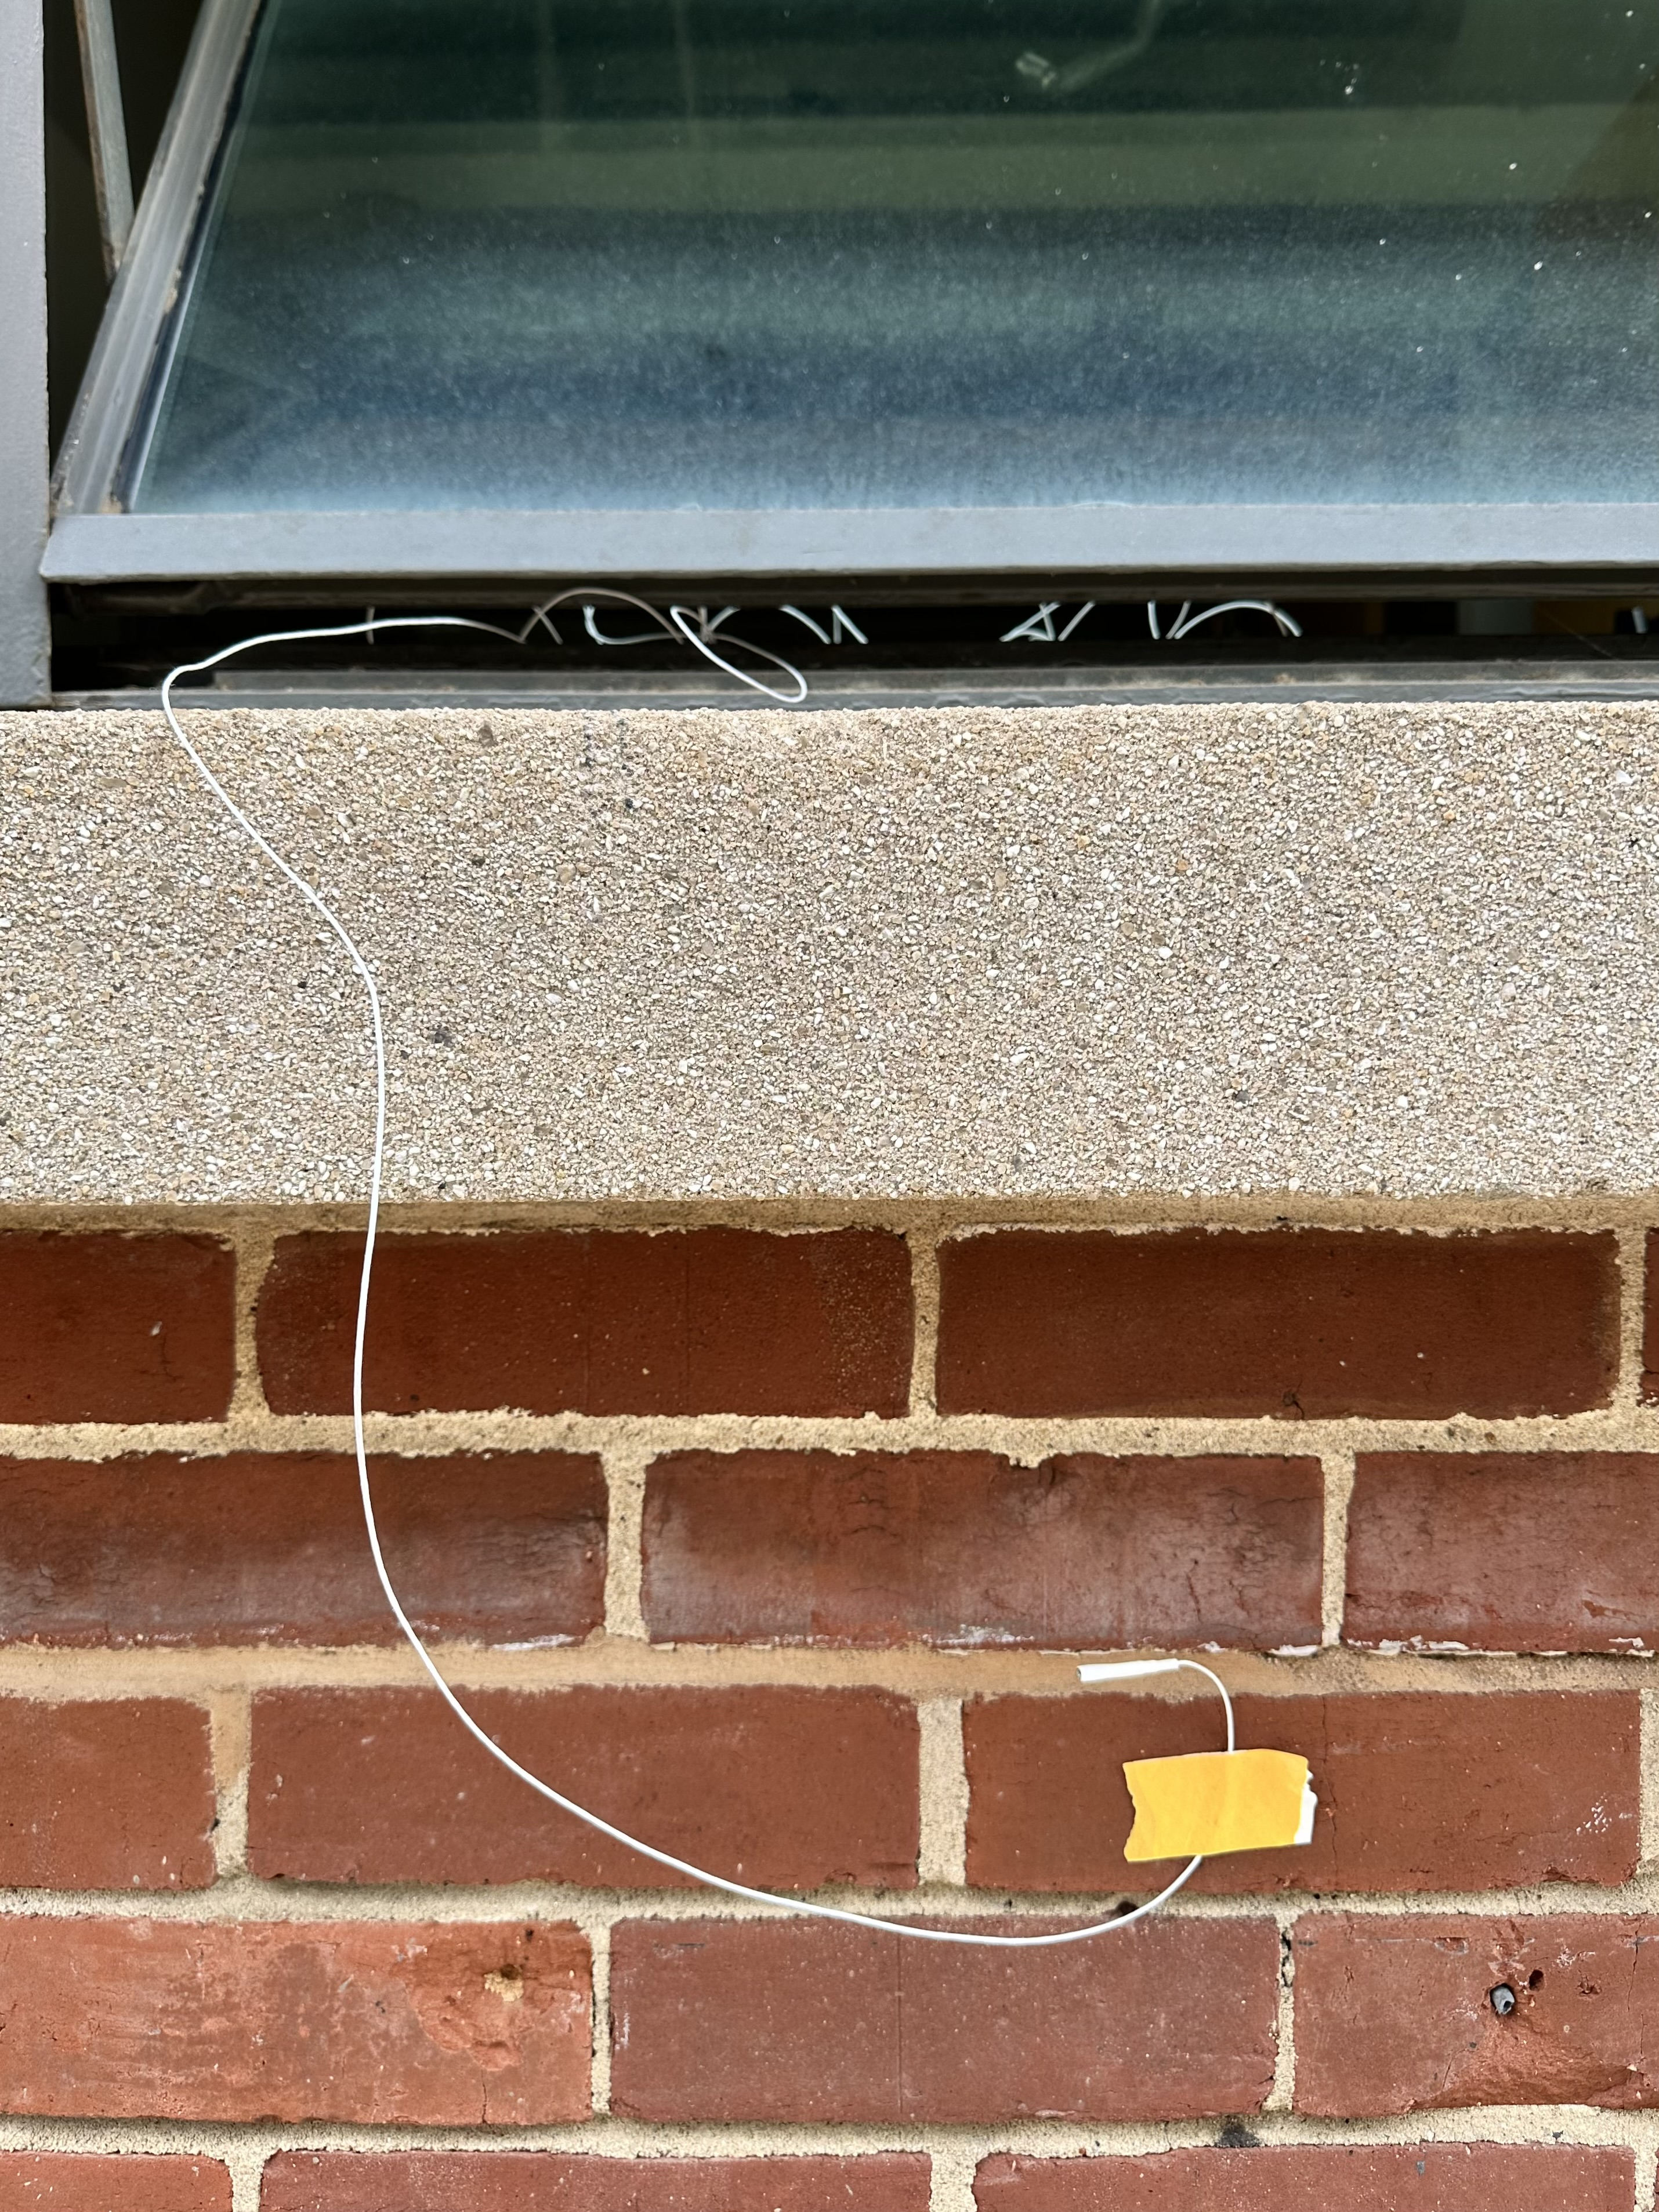
\includegraphics[width=0.495\linewidth]{Figures/expfig1.jpg}
    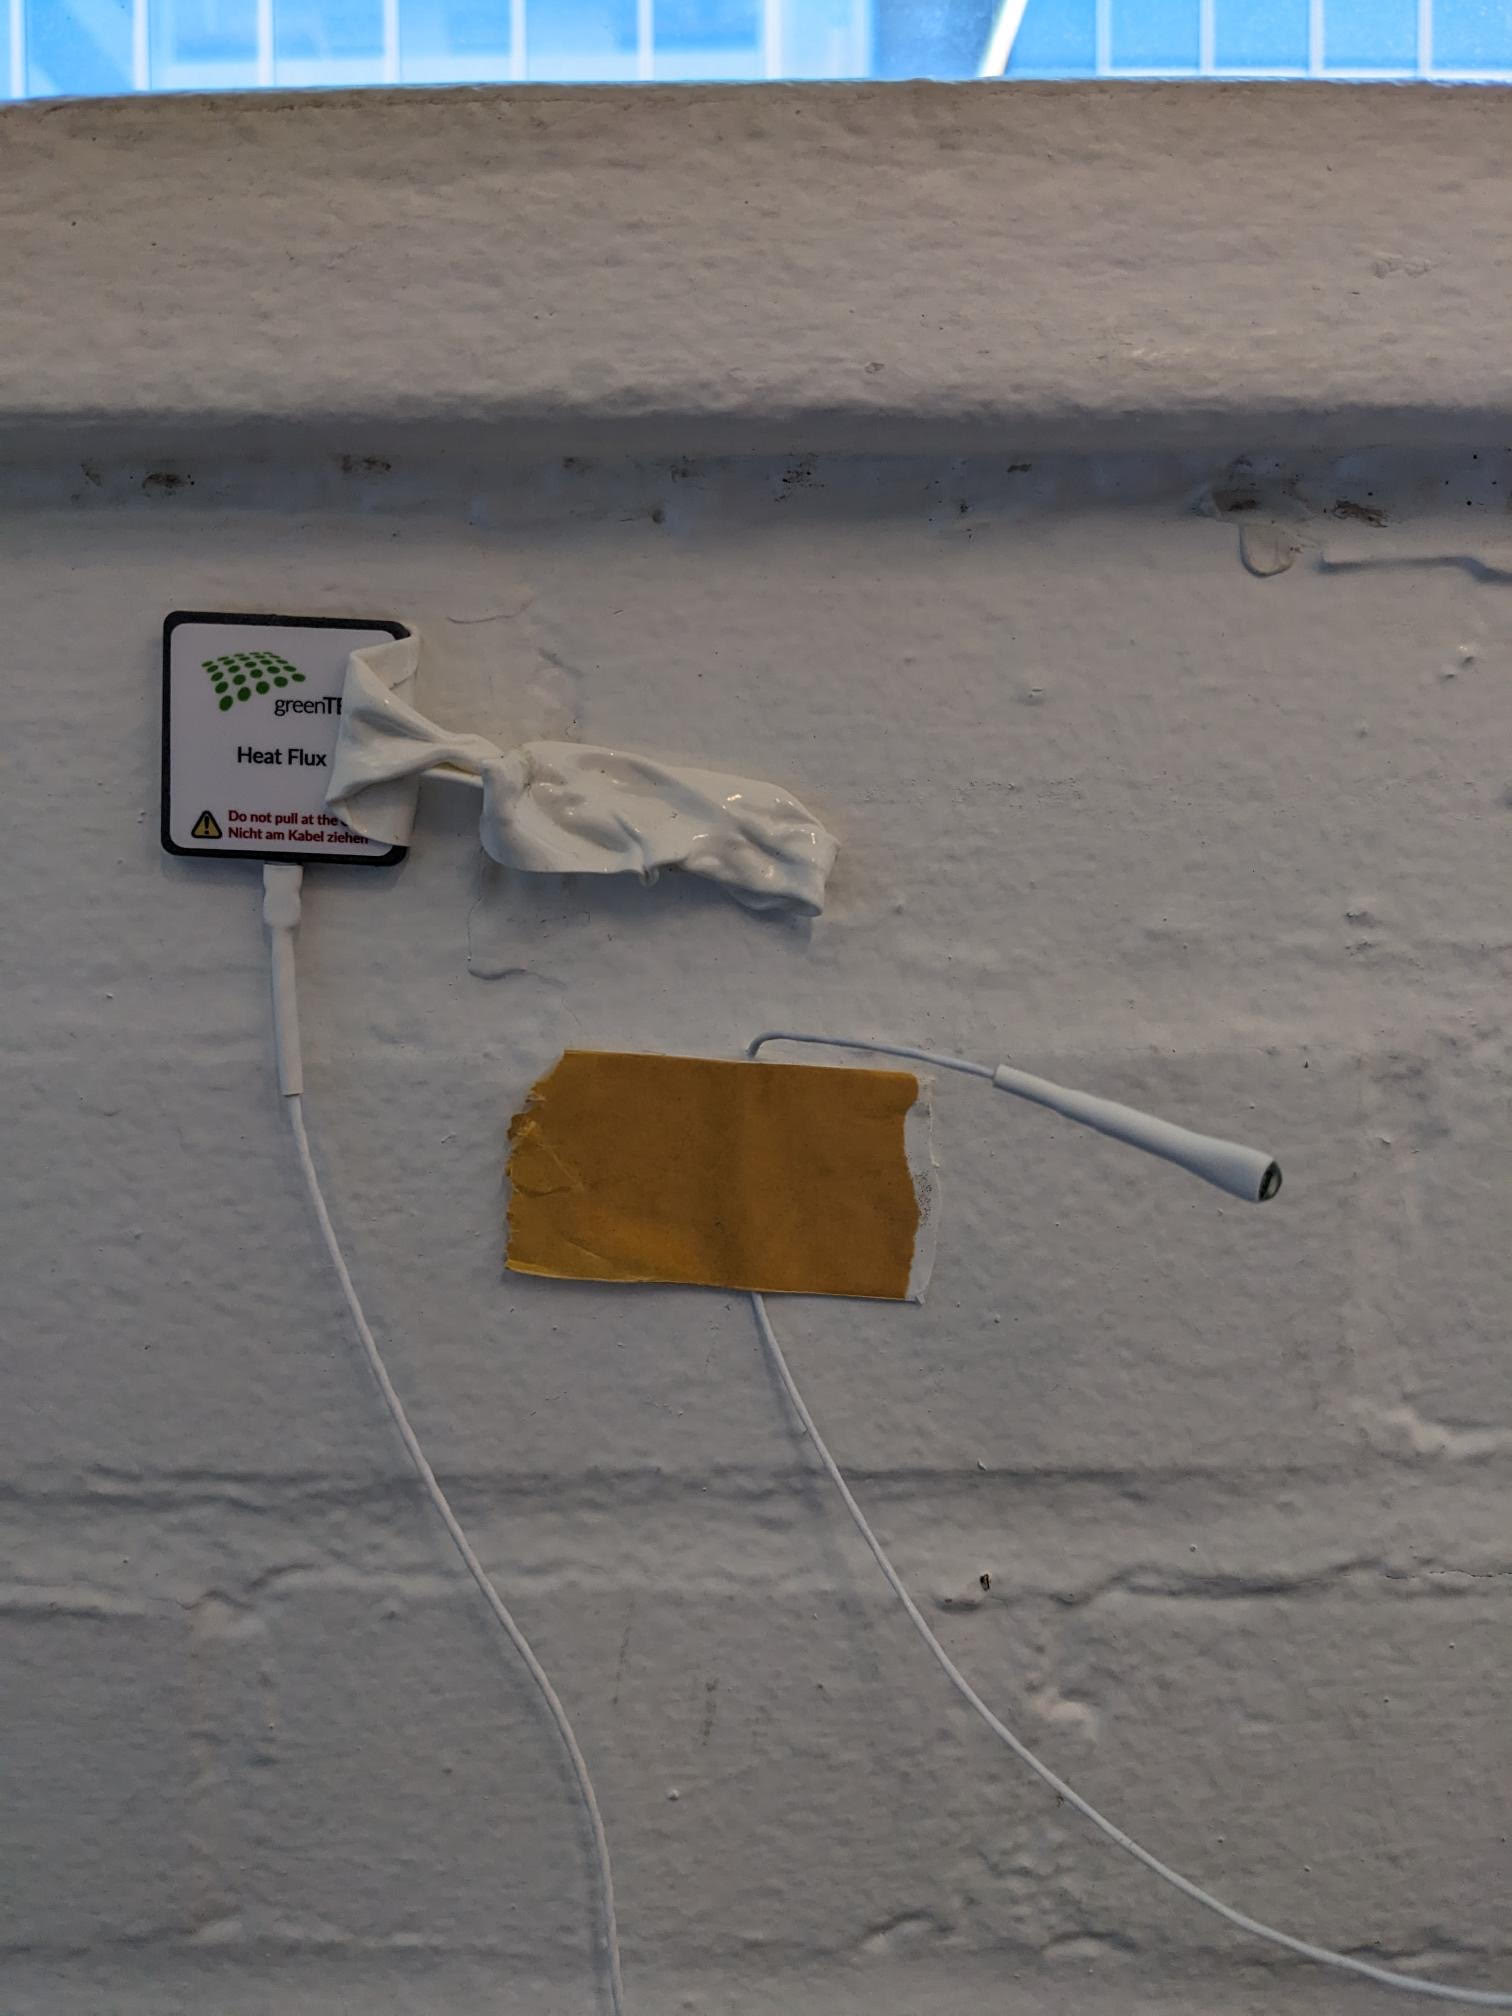
\includegraphics[width=0.495\linewidth]{Figures/expfig2.jpg}

    \hspace{3.5cm}\textbf{(a)}\hfill\textbf{(b)}\hspace{3.7cm}

     \caption[Experimental heat flux measurement setup]{Outdoor heat flux sensors during experimental design. The window was closed as much as possible to avoid interference with the sensor cord \textbf{(a)}. Indoor heat flux sensors during the experimental design \textbf{(b)}.}
   \label{fig:figexp1}
 \end{figure}




 
\subsubsection{Experimental Design}
 This experiment is based on using the measurement device used was the gSKIN® KIT-2615C (calibrated) U-Value and Heat Flux Measurement Kit from GreenTeg  \cite{greenteg} shown in \ref{fig:toolkit} and purchased by the funding received from Micro Research Grants for Regenerative Built Environments by  Kendeda Building Advisory Board \cite{kendeda}.
 \todo{fix this sentence}
 The schematic in \cref{fig:2d2} shows the experimental design setup with the same conditions of k  = 1 ${W/m}^2$ 
L  = 0.43 m,
$T_1$ = 25.8 $^\circ \text{C}$, 
$T_2$  = 21.1  $^\circ \text{C}$ .

\begin{figure}[tbh]
     \centering
    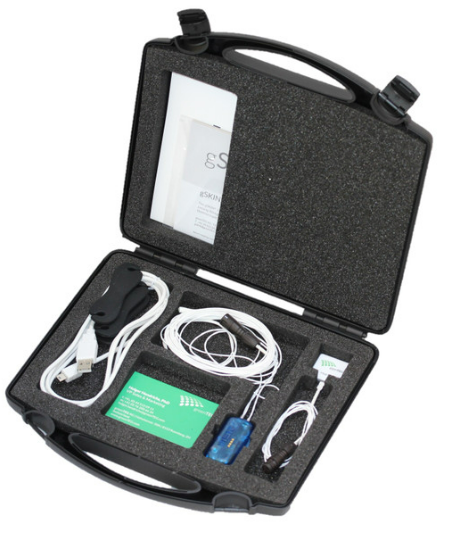
\includegraphics[width=0.5\linewidth]{Figures/greenteg.png}
     \caption[U-value measurement Kit]{The U-Value and Heat Flux Measurement Kit, for details see \cref{tab:u-value-measurement-kit}.}
   \label{fig:toolkit}
 \end{figure}






\subsubsection{Experiment Results}
This section showcases the results from sensor reading for the brick wall. The GreenTeg sensor company provides software to log and visualize the data, along with writing a final report with a CSV file documenting the reading on 10-second intervals. The chart in \ref{fig:expr} represents the temperature and heat flux results of the brick wall. 
The report indicates that the final resulting U value = 2.31 ${W/m^2k}$. Thus, according to the boundary conditions and the given results, the heat flux is \( q \) is \( 10.93 \, {W/m}^2 \). 
Where U-value from the report = 2.31 ${W/m^2k}$ and 
\begin{equation}
    U = \frac{k}{\text{L}}
      = \frac{1}{\text{0.43}} = 2.33  {W/m^2k}
\end{equation}
Where k = 1 \text{ W/(m²)}, L (thickness) = 0.43. So, \(U_{\text{calc}}\) = \(U_{\text{exp}}\) = 2.31 ${W/m^2k}$ 

\ref{fig:expr} below is a plot report showing the experimental design results of the fluctuations in indoor and outdoor temperature along with the heat flux. From the report, three temperatures from different time steps were selected to be compared with the 3D simulation results. Also, \ref{table2d} shows the comparison of the selected three points, where $T_{val}$ is the experiment's resulting temperature and $T_{sim}$ is the simulation's resulting temperature. 
The measurement approach represented in this section offers detailed time step values for temperature and heat flux. However, the cost of the sensor kit is considered high = \$2,157. Another issue with this approach is the time spent setting up and receiving results, where the minimum required reading time is 73 hours. Thus, the next section showcases an easier and faster method to find the heat flux, which using a 2D heat transfer simulation.

\begin{figure}[htb]
     \centering
    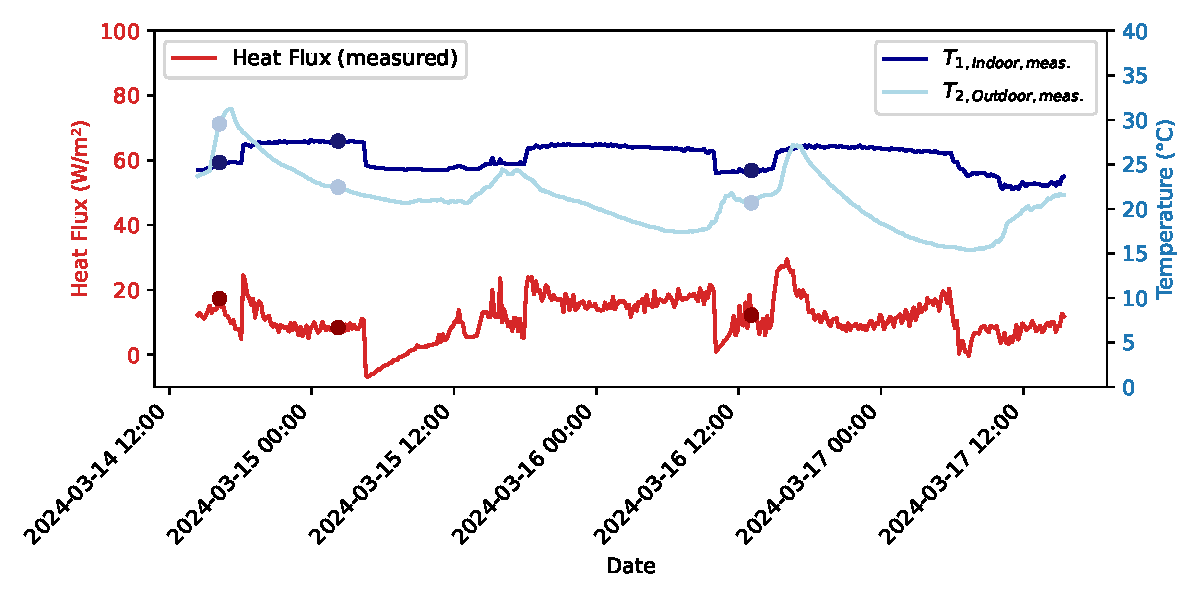
\includegraphics[width=1\linewidth]{Figures/Validation}
     \caption[2D Experimental Report Plot]{The line plots represent the sensor's heat flux and Temperature readings. where the points are the \gls{OF} simulation results.}
   \label{fig:expr}
 \end{figure}


\begin{table}[tbh]
    \caption{2D Temperature and Heat Flux Comparison}
    \label{table2d}
    \centering
    \begin{tabular}{lrrrrrrr}
        \toprule
        Time                & $T_{1,val,in}$ & $T_{1,sim,in}$ & $T_{2,val,out}$& $T_{2,sim,out}$ & $Q_{val}$ & $Q_{sim}$ \\
        \midrule
        3/14/2024 16:14 & 298.3    & 298.3    & 302.7     & 302.7     & 17.3 & 17.2 \\
        3/15/2024 02:14  & 300.7    & 300.7   & 295.5    & 295.6     & 8.9  & 8.3  \\
        3/16/2024 13:04 & 297.4  & 297.4   & 293.8   & 293.8   & 12.54 & 12.2  \\
        \bottomrule
    \end{tabular}
   
\end{table}




\begin{figure}[H]
  \centering
  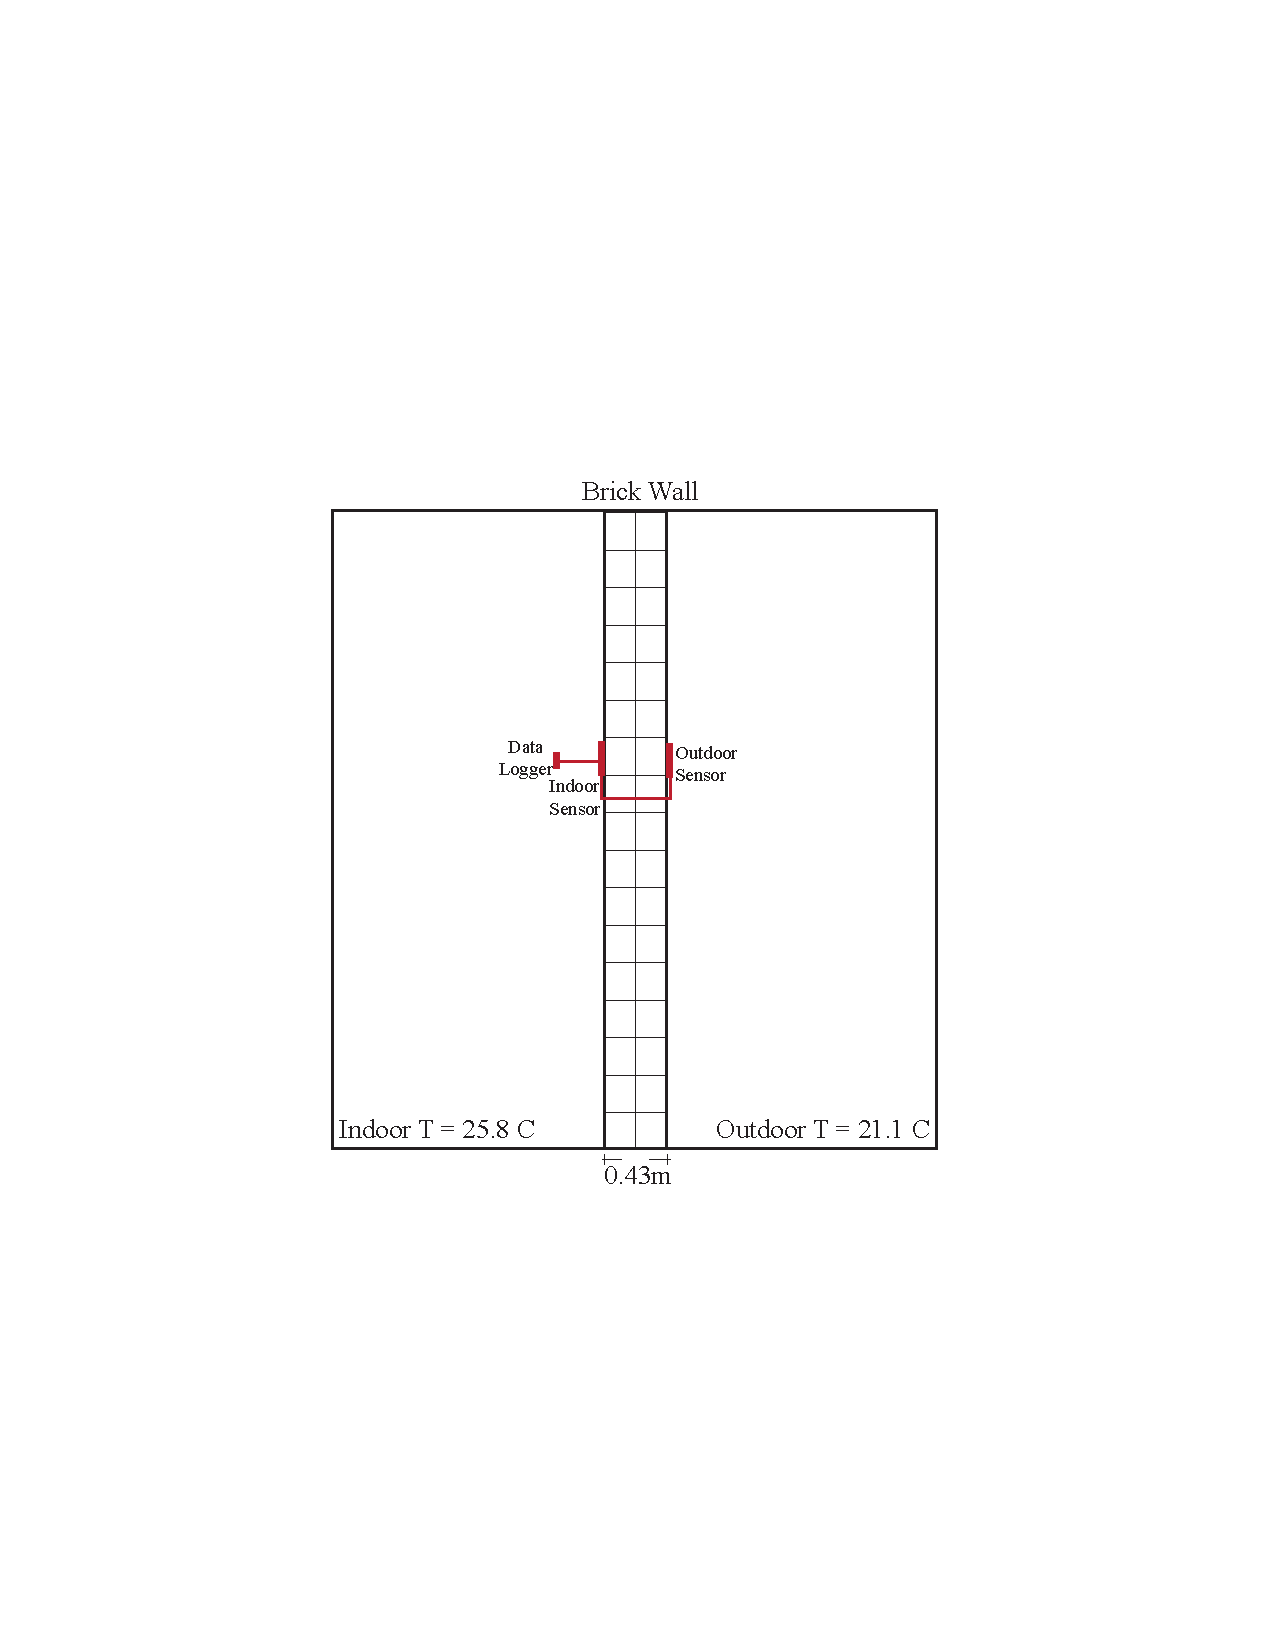
\includegraphics[trim=5.6cm 7.5cm 5.3cm 8cm, clip, width=.6\linewidth]{Figures/2dsection2.pdf}
\caption[2D Section and Setup]{Experiment setup for the 2D brick wall.}
\label{fig:2d2}
\end{figure}




















\section{Simulation}
\subsubsection{2D Simulation}
Moving to the third approach, which is using a 2D heat transfer software, where the same brick wall is modeled in HTFlux. HTFlux is a software that simulates 2D heat transfer seamlessly and calculates the heat flux with providing the temperature gradient \cite{HTflux}. The boundary conditions assigned in this simulation are the same as the previous methods which are ; brick thermal conductivity is k  = 1 ${W/m}^2$ 
L  = 0.43 m,
$T_1$ = 25.8 $^\circ \text{C}$, 
$T_2$  = 21.1  $^\circ \text{C}$ .


 \ref{2dconst} \textbf{(a)} which shows the materials and the boundary condition implemented in the software and \textbf{(b)} represents the 2D simulation results where the resulting heat flux = \( q \) is \( 10.91 \, {W/m}^2 \) as expected.










\begin{figure}[H]
\begin{minipage}{0.45\textwidth}
  \centering
  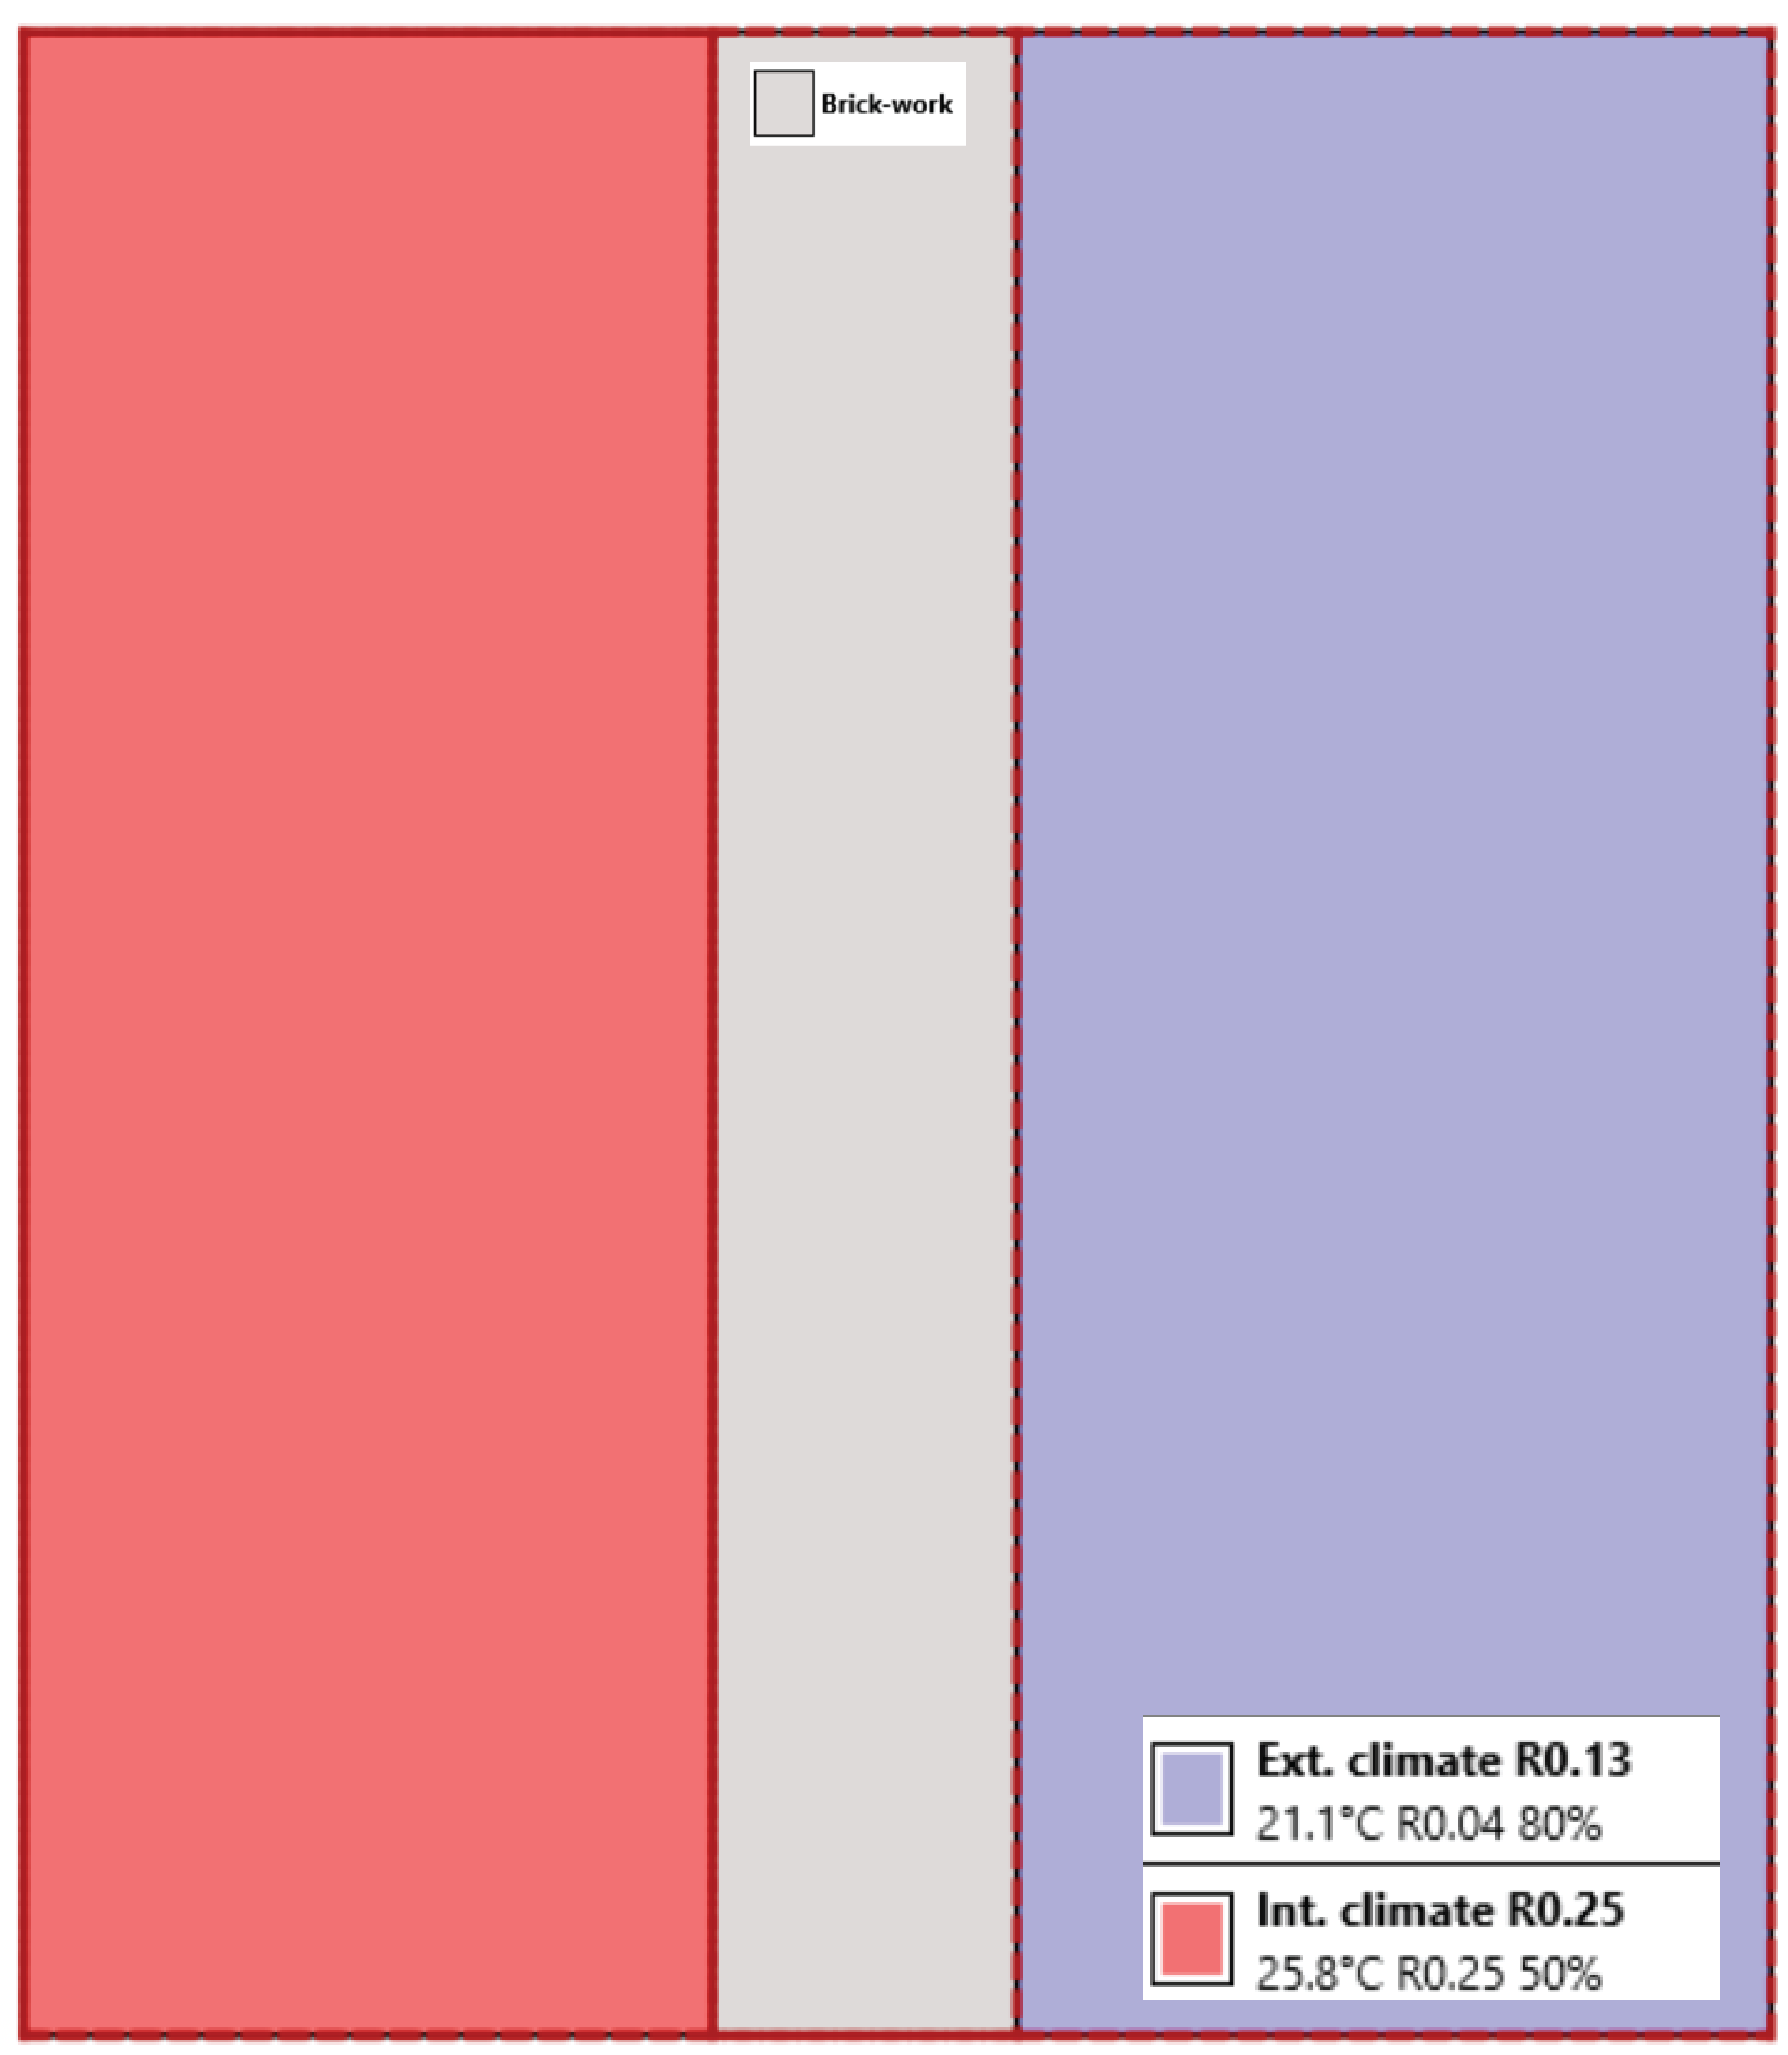
\includegraphics[width=\linewidth]{Figures/2dconst.png} 
  \caption*{\textbf{(a)} The simulation boundary conditions from HTFlux}
\end{minipage}%
\hspace{0.1\textwidth}
\begin{minipage}{0.45\textwidth}
  \centering
  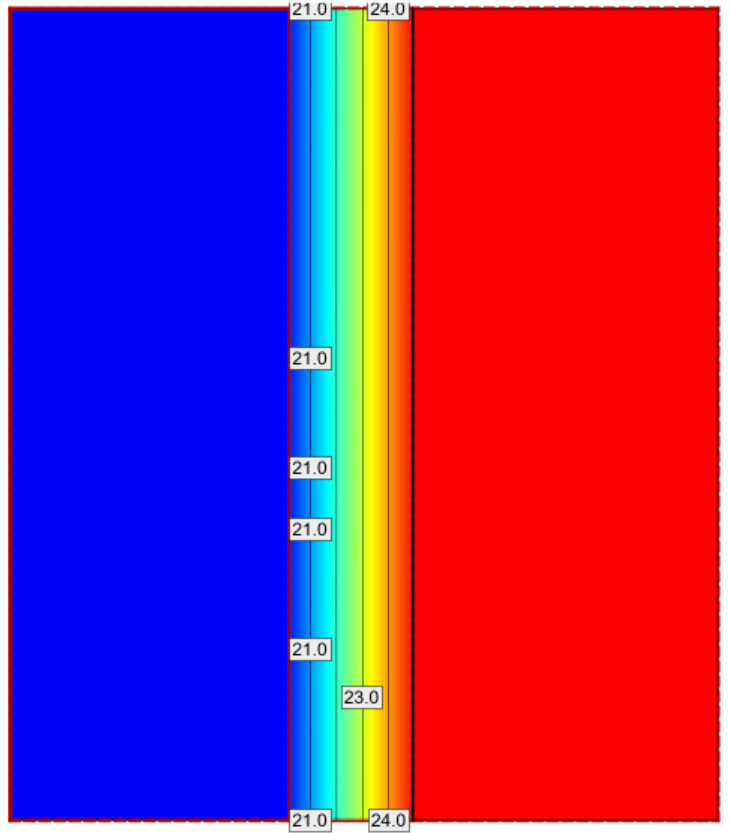
\includegraphics[width=\linewidth]{Figures/2dsim.png} 
  \caption*{\textbf{(b)} The brick wall temperature gradient results from HTFlux}
\end{minipage}
\caption{2D HTFlux Boundary conditions and Resulting heat flux of \( 10.91 \, {W/m}^2 \)}
\label{2dconst}
\end{figure}


\subsubsection{3D Simulation Compliance}\label{3dbrick}
Although chapter 4 explains the process of building the 3D heat transfer workflow in detail and validating the results with an ISO case, we returned to the brick wall in this chapter to model it with the 3D \gls{OF} simulation to further validate the results. So, the line plots in \ref{fig:expr} are the experimental design results and the points are the 3D heat transfer simulation results. \ref{error2d} is a comparison of the percentage of error between the results of the experiment and the 3D heat transfer workflow, where the average is from \%0.003 to \%0.01 and according to ISO\cite{ISO} to validate the case, the percentage of error shall not exceed \%0.1.


\begin{table}[H]
 \caption[2D Results Percentage error]{Percentage error demonstrating compliance between the experimental design results and the 3D workflow (in chapter 4) by calculating the percentage of error using the average method and the standard deviation method.}
    \label{error2d}
     \centering
 \begin{tabular}{l l l}
        \toprule
        Metric & T1 Percentage Error & T2 Percentage Error \\
        \midrule
        Average & 0.0032\% & 0.0102\% \\
        Standard Deviation & 0.0033\% & 0.0176\% \\
        \bottomrule
    \end{tabular}
\end{table}

\section{Discussion}
This section successfully presented the resources to calculate the heat flux of a 2D brick wall using three methods, which are by calculation, using sensors, using 2D simulation software where the heat flux q, respectively, = \( 10.93 \, {W/m}^2 \), \( 10.93 \, {W/m}^2 \), and \( 10.91 \, {W/m}^2 \). However, each of the presented approaches in this chapter are not convenient for an architect or a designer trying to seamlessly simulate 3D heat transfer. Thus, the gap of 3D heat transfer simulation integrated into the architecture modeling software is still missing and will be presented in the next chapter. In this chapter, \ref{3dbrick} is a work done after validating the 3D heat transfer tool, where the simulation is used to further validate the simulation using the brick wall example.
    
\chapter{3D Heat Transfer Methodology}

3D heat transfer simulation is a crucial aspect when designing, retrofitting, or analyzing an architectural envelope.
Simulation approaches enable modelers to understand and predict thermal comfort, providing detailed visualization of heat flow, insulation performance, and energy efficiency. 
Furthermore, 3D simulations are more accurate than the traditional methods highlighted in the previous chapter. 
In this way, users can detect and address complex issues such as thermal bridges and intricate geometric designs. 
This approach reduces the time, resources, and cost of identifying potential problems in the design of a building. 
 
This chapter showcases the workflow to build a 3D heat transfer approach integrated into architects' modeling software to precisely model and optimize building envelopes, leading to better informed decisions about insulation, material choice, and energy efficiency. The flowchart in \ref{fig:flowchart} is an overview of the 3D simulation steps. The following sections present the validation case, methodology, pre-processing, simulation setup, solver explanation, automation, post-processing, results, and finally the discussion. 






   
\begin{figure}[h!]
     \centering
    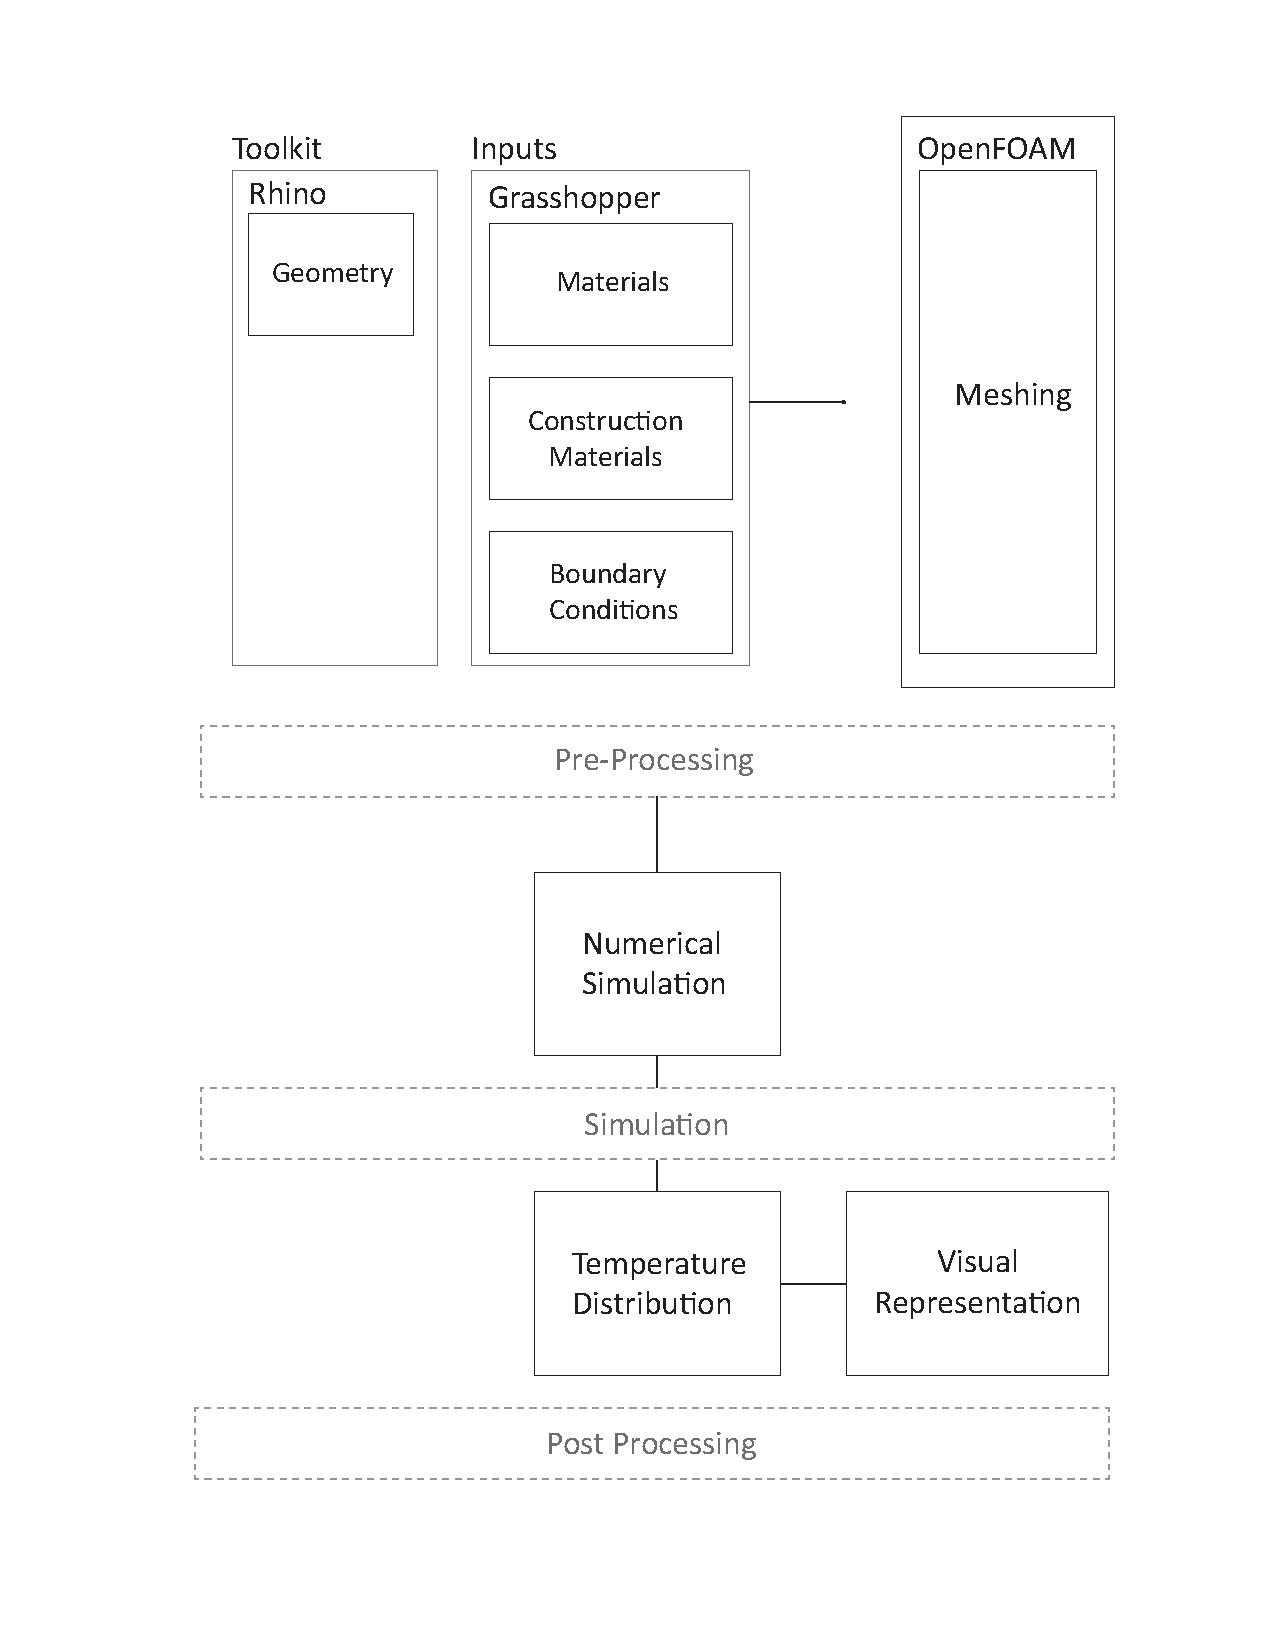
\includegraphics[trim=2.7cm 1.7cm 2.7cm 1.5cm, clip, width=0.7\linewidth]{Figures/flowchartv.pdf}
     \caption[Simulation Flowchart]{Flowchart of simulation steps starting from pre-processing to the post-processing of the simulation.}
   \label{fig:flowchart}
 \end{figure}



\subsubsection{Methodology Overview}
The first step in the methodology is to select a 3D validation case study to model in Rhino. 
Then, \gls{GH}  is used to create a script that bridges the gap between Rhino (the architectural modeling software) and  \gls{OF} (the CFD software package). A detailed description of the workflow, \gls{GH} automation, and the \gls{OF} solver are illustrated in the following sections.





\section{Validation Case Study}
The selected case comes from the International Organization for Standardization (ISO) \cite{ISO}. The case study is a validated 3D heat transfer case documented in \textit{ISO 10211:2007}\footnote{ISO 10211:2007---Thermal bridges in building construction. Validation of case A.3 \cite{ISO}.}. 
The geometry consists of two levels: a first floor and a second floor, separated by a floor slab and a plaster floor. The walls are composed of aerated concrete, insulation material, and brick.
A description of each material in the geometry can be found in \ref{fig:validation-case-materials} \textbf{(a)}.

%One of the challenges we faced was retrieving this case study due to the lack of availability of validated 3D and not 2D heat transfer cases that incorporate building materials. 
Beyond \textit{ISO 10211:2007}, it is also documented in QuickField 6.6 (student version) software where the properties, layers, and boundary conditions of the materials are accessible, which we exported to compare it with our method. 

   


\begin{figure}[h!]
    \centering
    \begin{minipage}[t]{0.54\columnwidth}
        \centering
        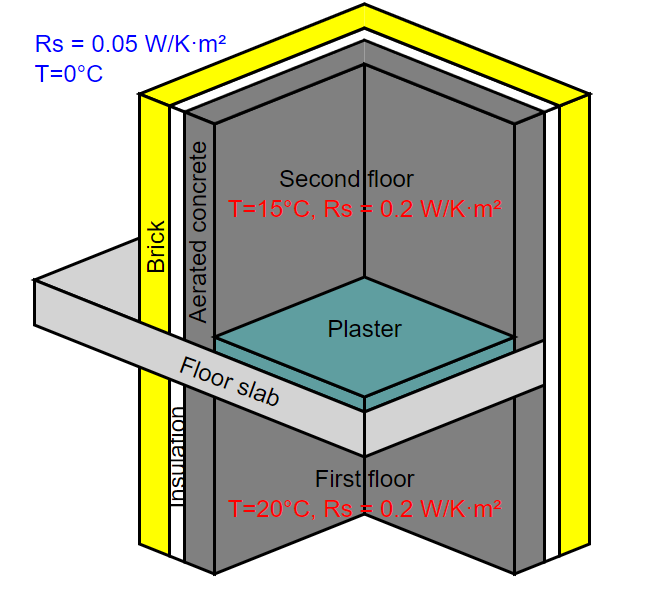
\includegraphics[width=\linewidth]{Figures/validationcase}
        \textbf{(a)}
    \end{minipage}
    \hfill
    \begin{minipage}[t]{0.8\linewidth}
        \centering
        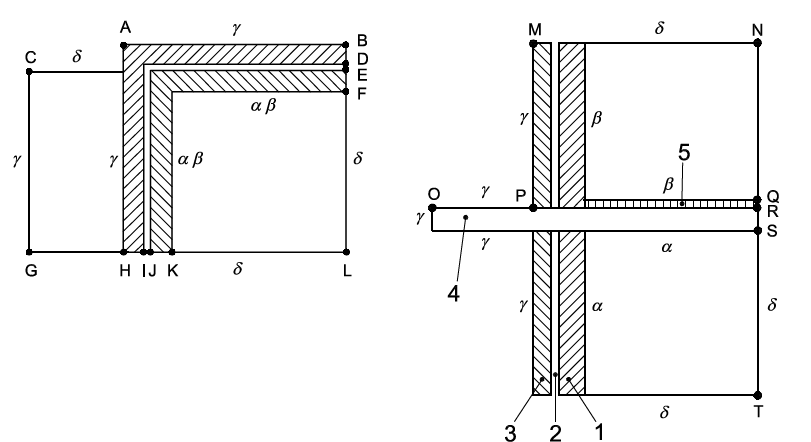
\includegraphics[width=\linewidth]{Figures/isodesc.png}
        \textbf{(b)}
    \end{minipage}
    
    \caption[3D Validation Materials]{\textbf{(a)} Validation case materials \cite{ISO}. \textbf{(b)}  Validation case sections retrieved from \gls{EN} ISO 10211:2007(E) \cite{ISO}.}
    \label{fig:validation-case-materials}
\end{figure}









QuickField's Heat Transfer module offers versatile features including steady-state and transient formulations with customizable initial field distributions and flexible time parameters, accommodating nonlinear specific heat and nonlinear or anisotropic properties. Although the results include diverse thermal field mappings such as temperature, heat flux, and thermal gradients, editing and customizing the post-process options and locations were limited.




\section{Rhino  Automation} %STOPPED HERE
After selecting the validation case, the geometry is modeled in Rhinoceros, where it will be used as a user interface to connect the model to \gls{GH}. \gls{GH} is a visual programming environment that we use to automate the \gls{OF} simulation. 
The \gls{GH} script enables the automation of the geometry pipeline, which, for example, enables us to find the coordinates of the points in the region and to set the mesh, boundary conditions, and material properties. 
In addition, we use \gls{OF}, which is an open-source computational fluid dynamics (CFD) software package that is used to simulate fluid flow, heat transfer, and other capabilities. 


%\subsection{OF Text files Automation by  \gls{ \gls{GH}}}   
This subsection explains the Grasshopper script that automatically creates and exports STL files, defines material properties, finds the location of the points in the meshes, and writes all the text files needed to run the \gls{OF} case.

\subsubsection{Materials Properties Component}
The component shown in \ref{matgh} is a dictionary for the material connected to a specific geometry. Each different zone in Rhino needs to be connected to the shown component by adding the corresponding specifications for the material such as name, type, temperature, specific heat capacity, thermal conductivity, and density. This component is considered the base, and many other sections in the script depend on it, such as writing the other text files in 0 files where the boundary conditions are needed or writing the constant and system files. 


\begin{figure}[tbh]
\centering
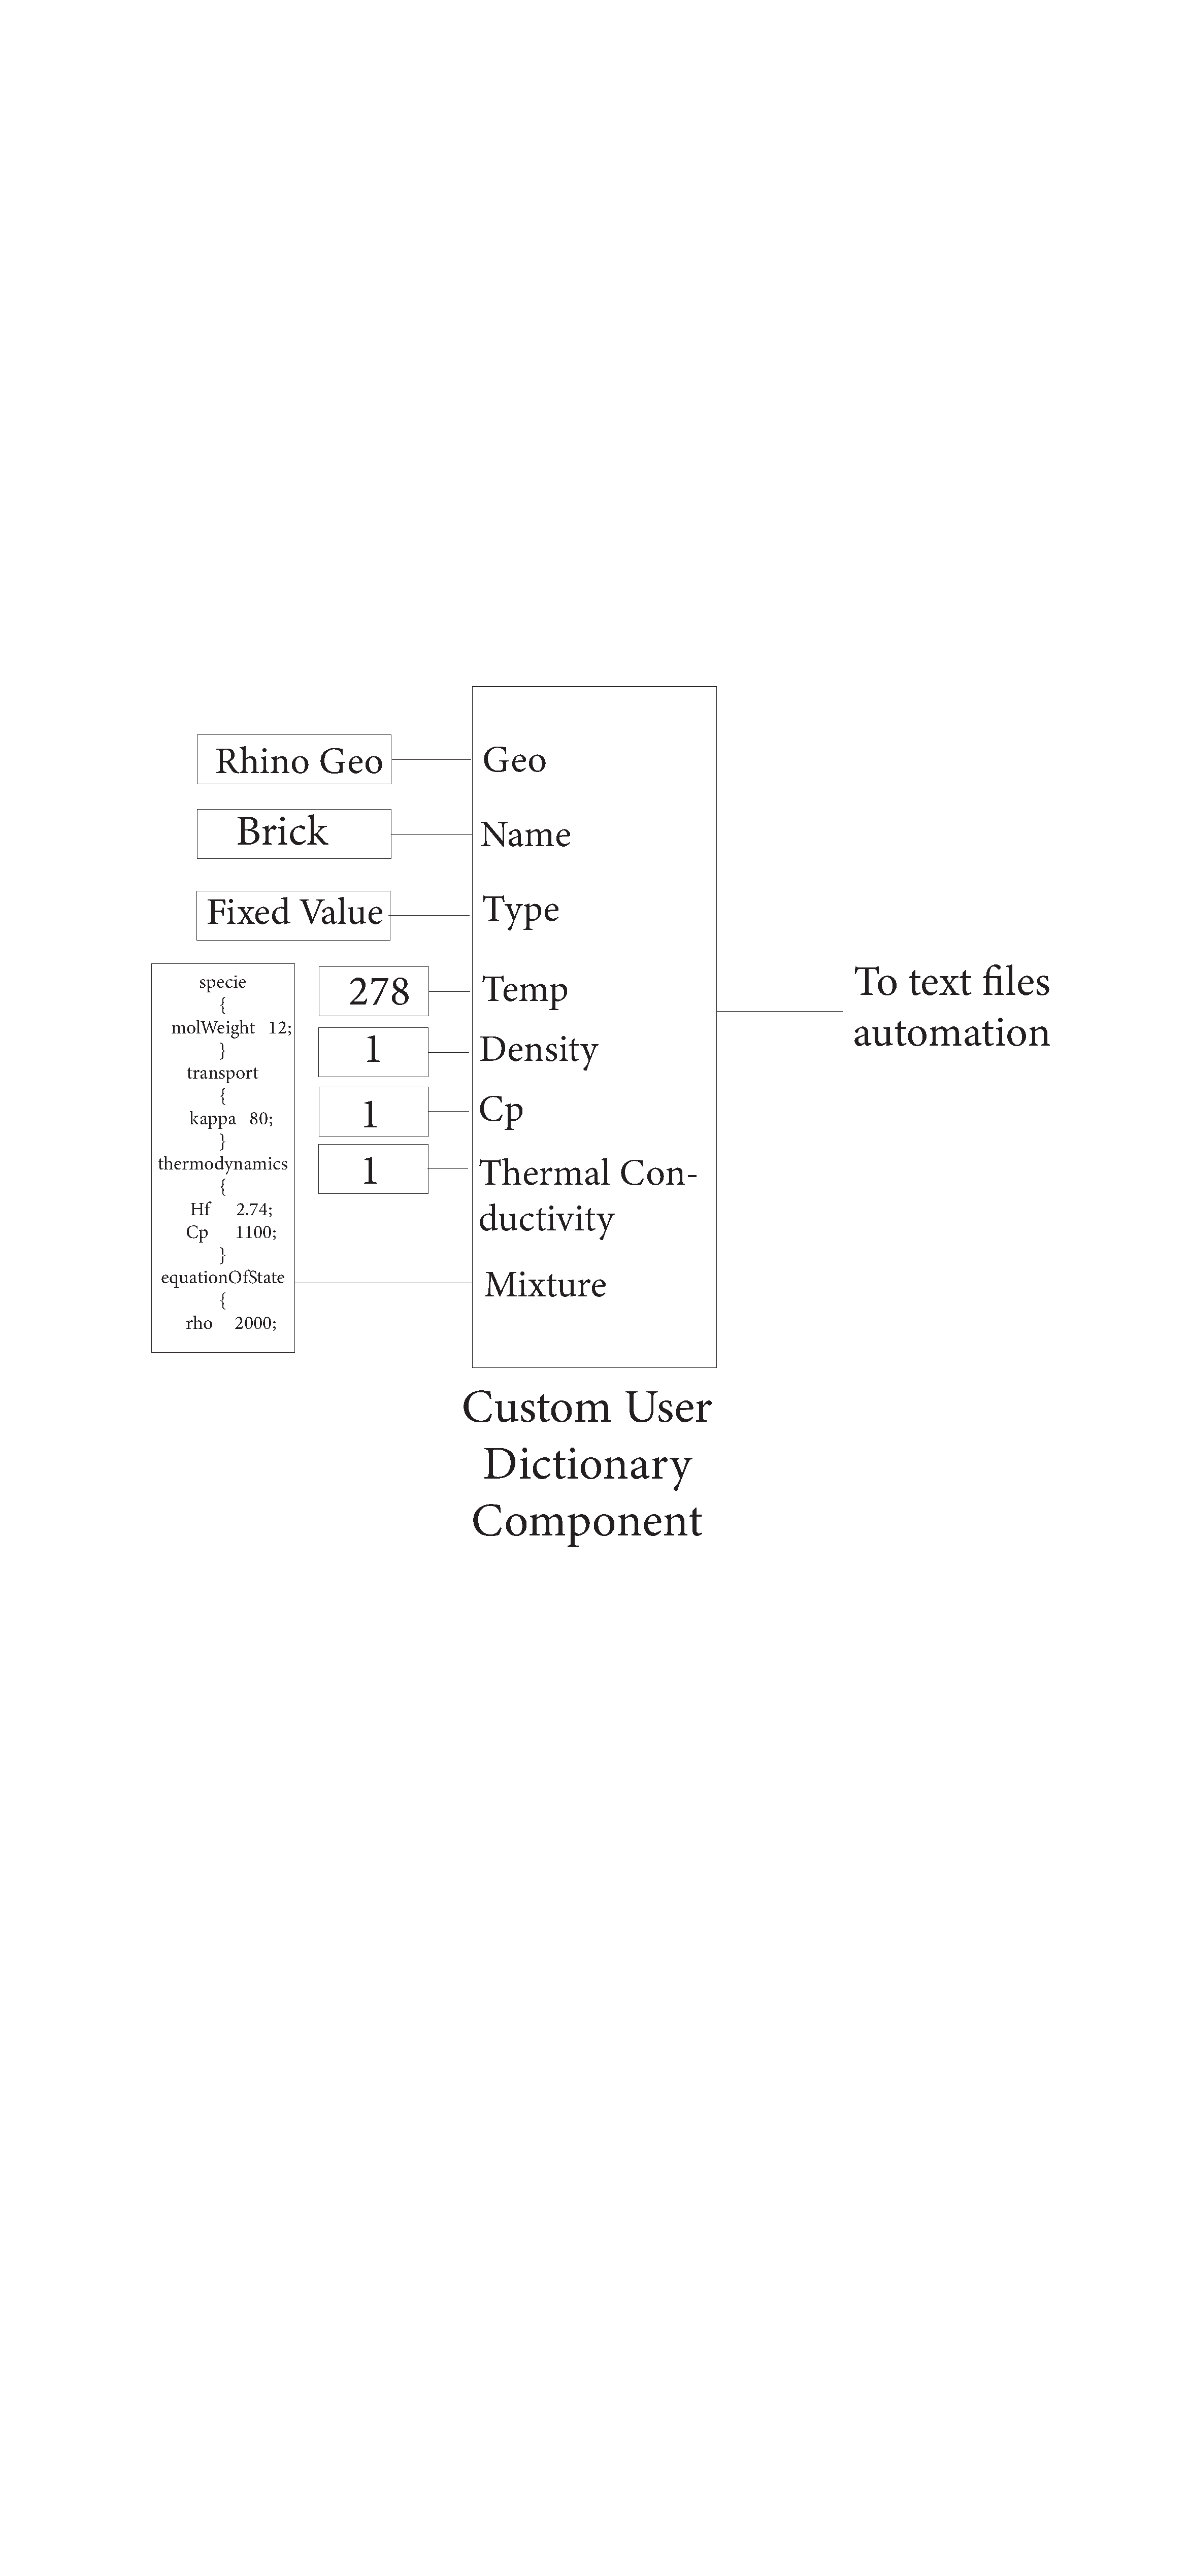
\includegraphics[trim=5cm 32cm 4.5cm 7cm, clip, width=0.55\linewidth]{Figures/THESISGH2.pdf}
\hspace{0.7cm}
\caption{\gls{GH} Material Properties Component.}
\label{matgh}
\end{figure}





\subsubsection{\gls{GH} Point in Mesh}
The workflow in \ref{locgh} automatically defines the point coordinates of each region of the mesh. Each region must have a point in Rhino, and the points of each are connected to the corresponding material component. The \textit{locationInMesh} parameter identifies a specific point within the computational domain, allowing the \textit{snappyHexMeshtool} to identify and locate all cells connected to that point. This helps ensure that only certain regions/zones are kept during the mesh generation process, usually to separate different volumes or regions of interest.

In our case, one point is not enough to capture all 10 regions, so using \textit{locationsInMesh} is essential. This allowed us to specify a list of points that represent various locations within the mesh. Each point in this list creates a separate cell zone located in the \textit{constant/ConcreteTop/polyMesh/cellZones} file, allowing more complex meshing and region differentiation. This flexibility is useful for our case and for other complex geometries within a single mesh.

\begin{figure}[tb]
\centering
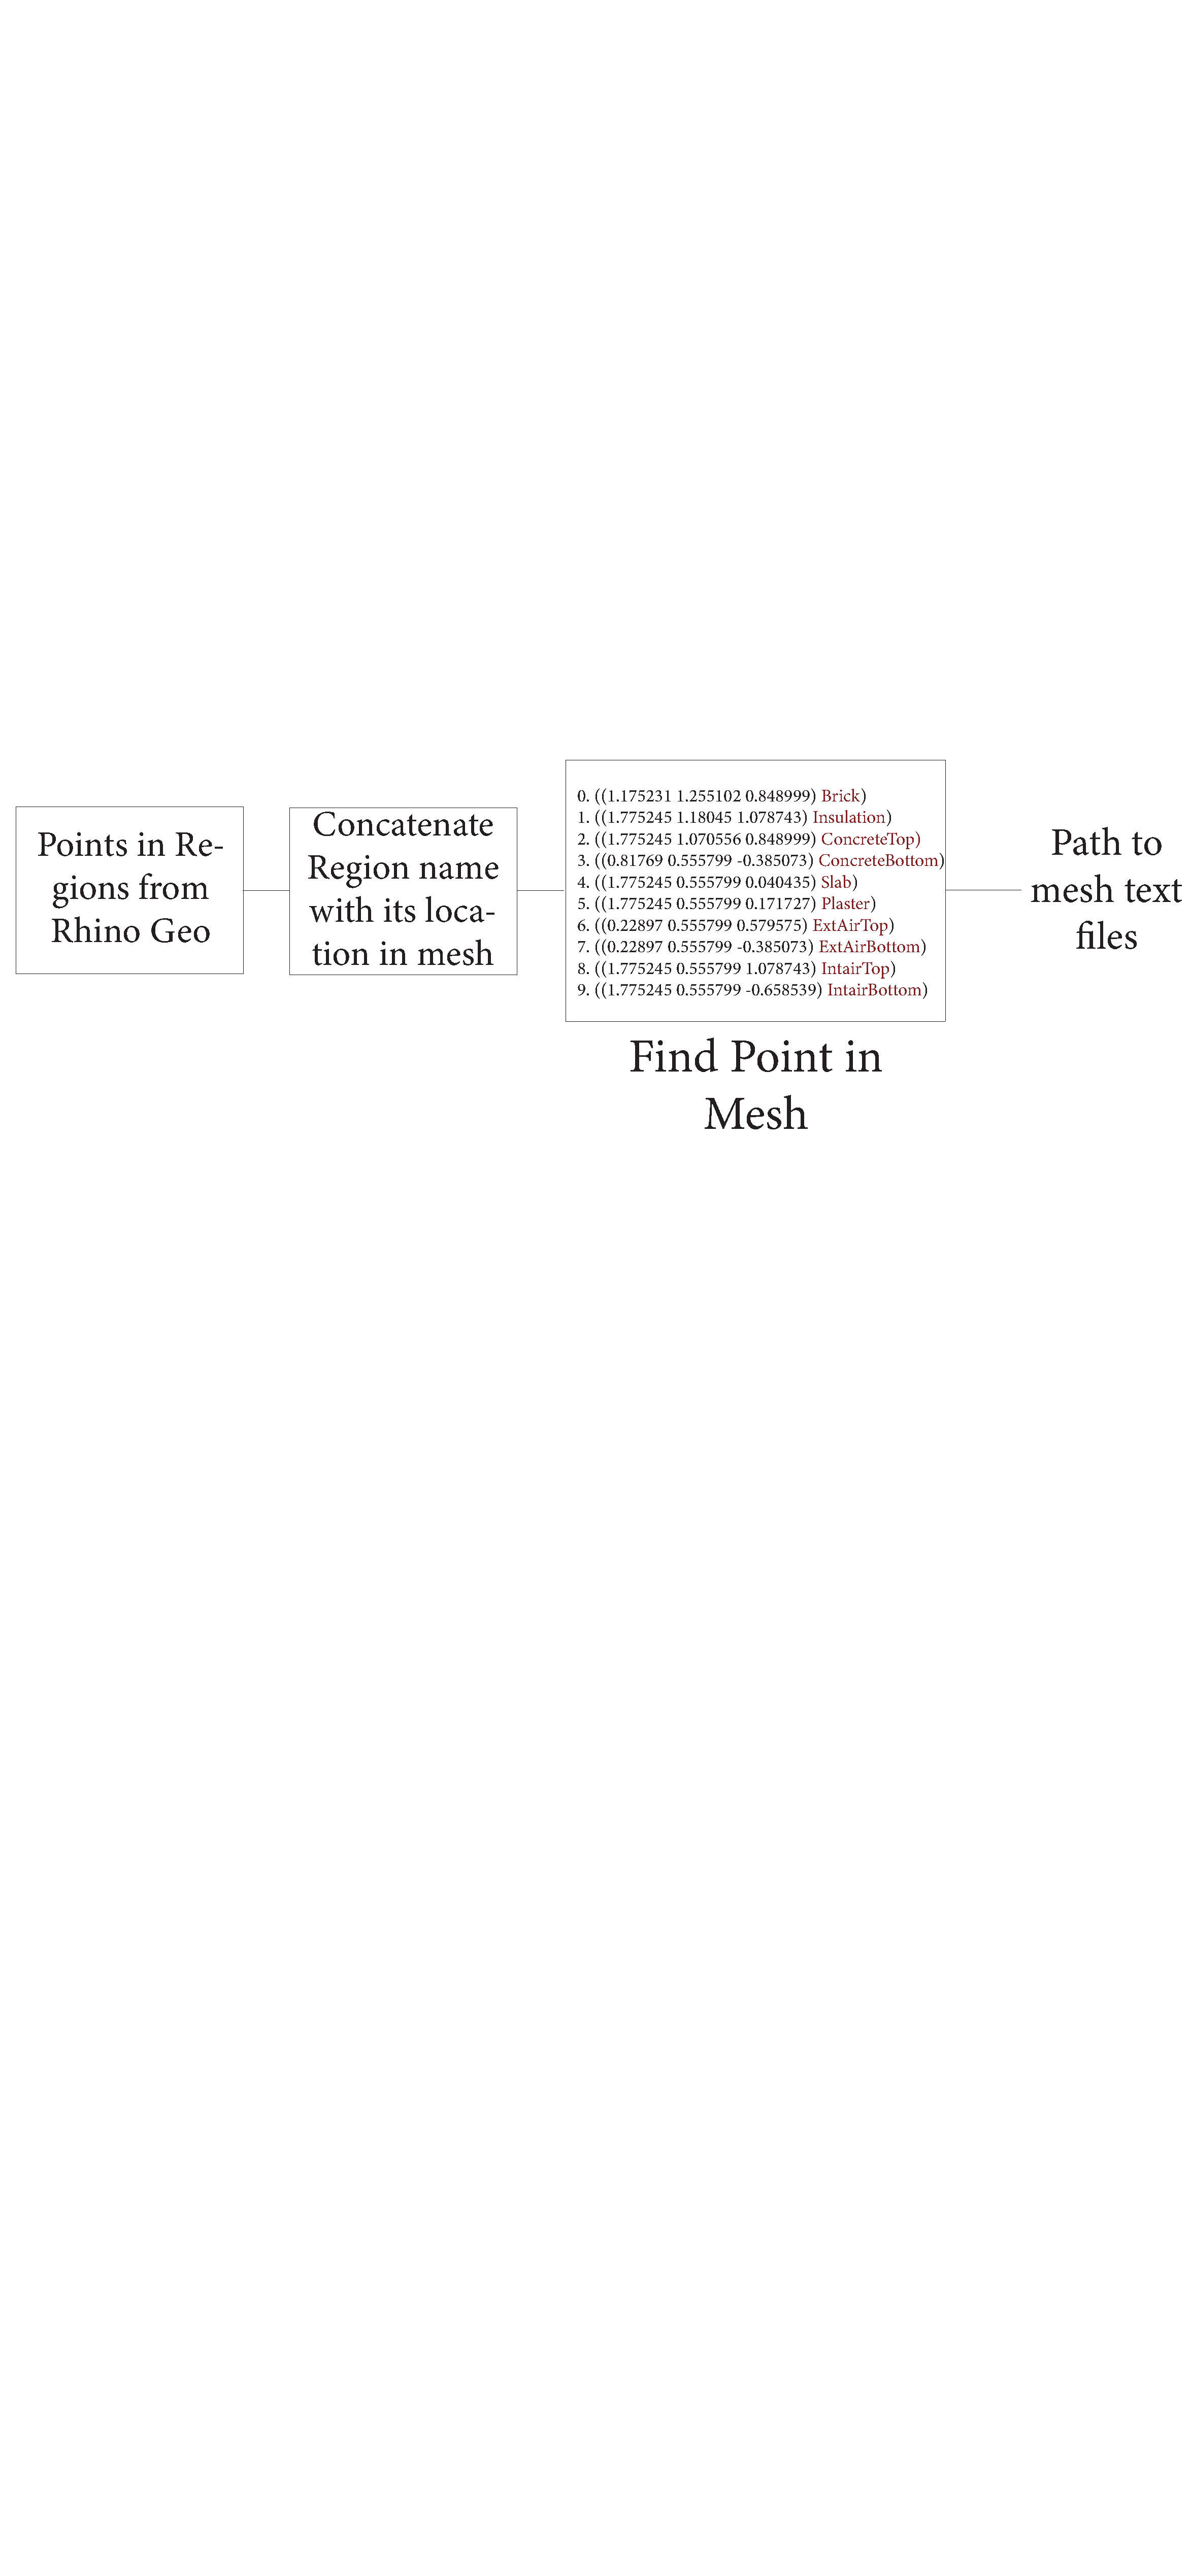
\includegraphics[trim=0cm 45cm 0cm 24cm, clip, width=0.8\linewidth]{Figures/locinmeshgh.pdf}
\hspace{0.7cm}
\caption{\gls{GH} Point in Mesh Workflow.}
\label{locgh}
\end{figure}








\subsubsection{Surface Combinations}
The surface combinations workflow shown in \ref{surfgh} writes the zone interfaces to be used in each zone text file in \textit{constant}, \textit{system}, and \textit{0}. 

\begin{figure}[tb]
\centering
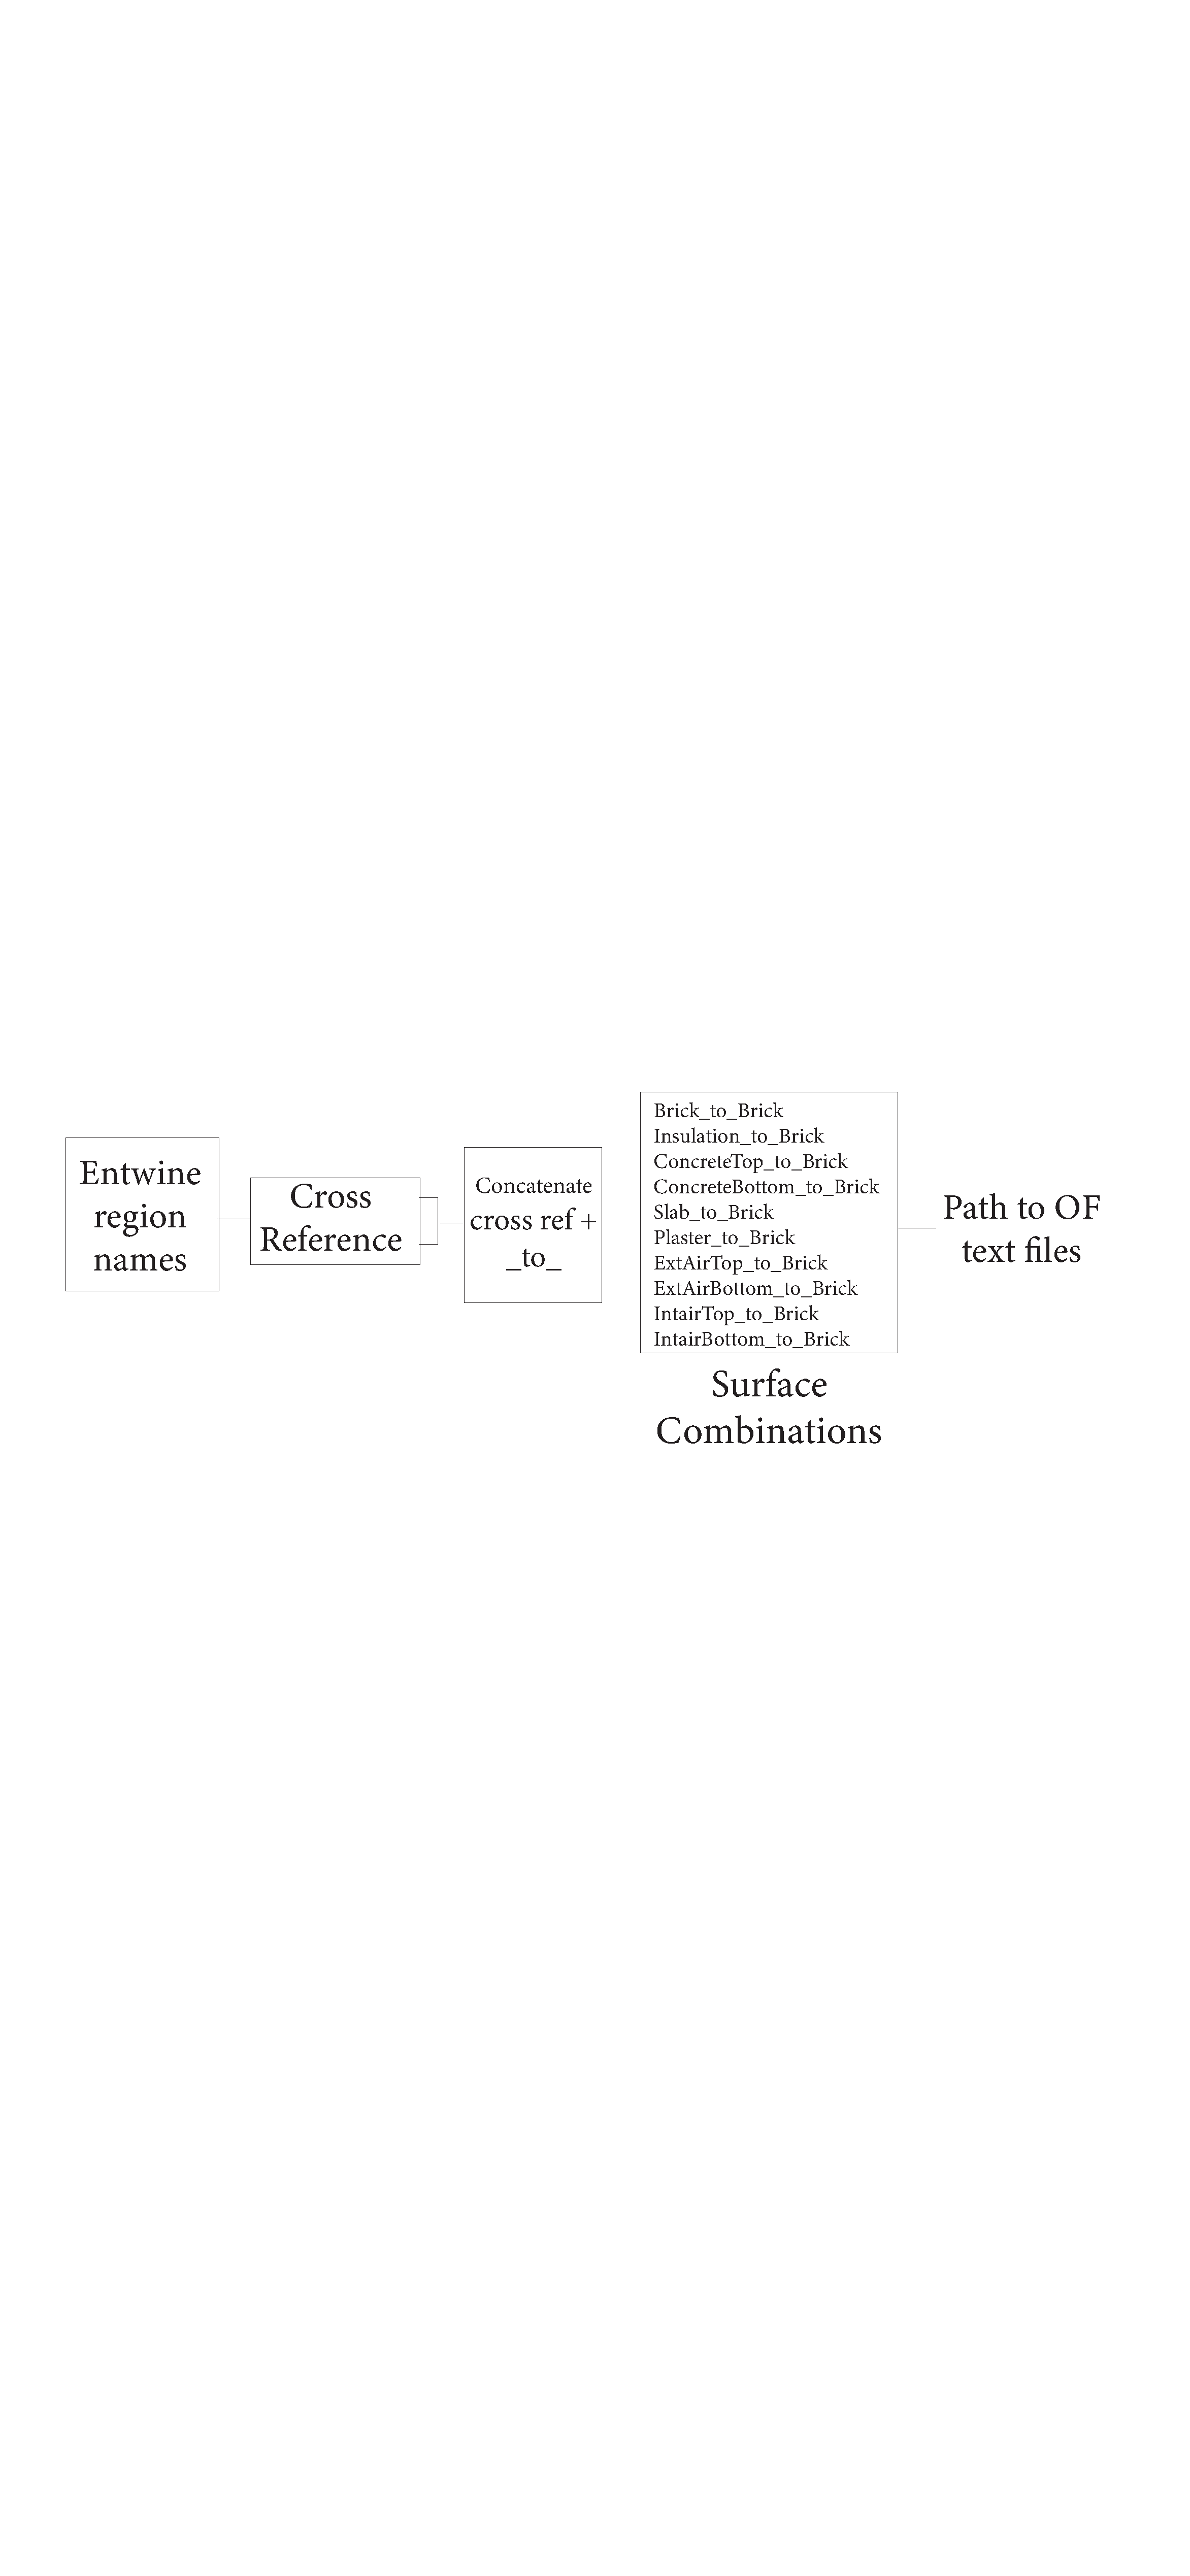
\includegraphics[trim=0cm 39cm 0cm 29cm, clip, width=0.8\linewidth]{Figures/surfcombgh.pdf}
\hspace{0.7cm}
\caption{\gls{GH} Surface Combinations Workflow.}
\label{surfgh}
\end{figure}



\subsubsection{Write p File Example}
The \gls{GH} script includes sections to write all of the $p$, $T$, $U$, and properties files needed to run the simulation for each zone. All other required text files, such as T and U, are written using the same workflow where the component includes a script that writes the text file in the required format \gls{OF}. Furthermore, all the necessary boundary conditions and material specifications are taken from the material dictionary component in \cref{matgh}.


















\section[OpenFOAM]{OpenFOAM (OF)}
As briefly stated at the beginning, this project utilizes the CFD capabilities of OpenFOAM (Open-source Field Operation and Manipulation, or OF).  \gls{OF} is a C++ toolkit built for developing custom numerical solvers and pre- and post-processing tools. \gls{OF} is mainly used to simulate computational fluid dynamics (CFD). The software is open-source, free to use and is distributed under the GNU General Public License Version 3.
By integrating the capabilities of \gls{OF} into Rhino, the complexity of setting up a 3D heat transfer case is simplified and minimized. When using OpenFOAM for simulations, it is important to note that the temperatures for boundary conditions must be specified in Kelvin.

This section provides a detailed description of the case's pre-processing, case study setup, selected solver, and physical models, as well as a description of constructing and running the case. 
Finally, it provides detailed post-processing steps.



\subsection{Pre-processing}
The pre-processing phase consists of dividing the geometry into different zones based on different materials and locations. In addition, thermophysical properties, such as specific heat capacity and thermal conductivity, are assigned to the materials, and fluid or solid properties are assigned to regions. The limit conditions and the construction materials are specified in \cref{fig:validation-case-materials} \textbf{(a)} and \textbf{(b)}. 


\begin{figure}[h!]
    \centering
    \begin{minipage}[t]{1\columnwidth}
        \centering
        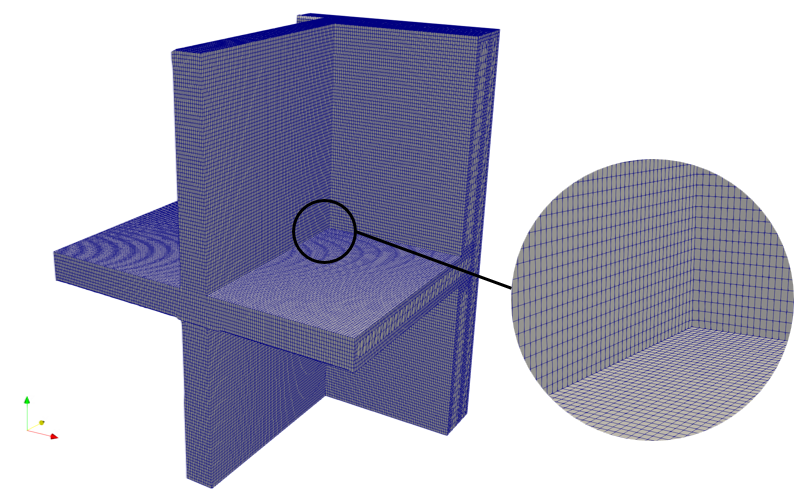
\includegraphics[width=\linewidth]{Figures/mesh3.png}        
        \subcaption*{\textbf{(a)}}
        \vspace{0.5cm}
    \end{minipage}
    
    \begin{minipage}[t]{0.5\columnwidth}
        \centering
        \begin{tabular}{clrrr}    
            \toprule
            & Type       & Multi-block dataset   \\ \midrule
            & \# of Cells & 360,364                      \\
            & \# of Points                        & 3,481,036                  \\
            & \# of TimeSteps                  & 400                        \\
            & Bounds X          & 0 to 1.9 (delta: 1.9) \\
            & Bounds Y          &                     0 to 1.25 (delta: 1.25) \\
            & Bounds Z          &                     -1 to 1.15 (delta: 2.15)    \\  \bottomrule
        \end{tabular}
        \caption*{\textbf{(b)} 3D Validation case mesh statistics.}
        \label{tab:mesh-stats}
    \end{minipage}
    
    \caption[3D Validation Mesh and Mesh Statistics]{\textbf{(a)} \gls{OF} mesh viewed in ParaView without air regions. \textbf{(b)}  Validation case mesh statistics retrieved from ISO 10211:2007 (E) \cite{ISO}.}
    \label{fig:validation-case}
\end{figure}






\begin{table}[tbh]
    \centering
    \label{tab:construction_material_properties}
    \caption[3D Material Properties]{Construction material properties and boundary conditions used for the simulation domain. Data were taken from the demo example in QuickField.}
      \centering
        %\footnotesize
        \begin{tabular}{clrrr}    
            \toprule   
            & Materials       & $k$ $\left[ \si[per-mode=fraction]{\watt\per\metre\kelvin} \right]$ & $c_p$   $\left[ \si[per-mode=fraction]{\joule\per\kilogram\kelvin}\right]$ & $\rho$  $\left[ \si[per-mode=fraction]{\kilogram\per\cubic\metre} \right]$   \\
            \midrule
            & Floor Slab        & 2.5                        & 1000                      & 2300               \\
            & Aerated Concrete  & 2.5                        & 1000                      & 2300               \\
            & Brick             & 0.7                        & 1060                       & 710               \\
            & Insulation        & 1                         & 1450                      & 35               \\
            & Plaster           & 1                         & 1000                      & 2300              \\
            \bottomrule
        \end{tabular}
  
\end{table}


    \begin{table}[tbh]
   
      \caption{3D Boundary Conditions}
      \centering
        %\footnotesize
        \begin{tabular}{llrr}    
            \toprule   
            & Boundary conditions          & $T [\si{\degreeCelsius}]$           & BC type                   \\ 
            \midrule
            & Inside temp.  (1st floor)         & 20                          & fixedValue                \\
            & Inside temp.  (2nd floor)          & 15                          & fixedValue                \\
            & Outside temp.  & 0                          & fixedValue                \\ 
            \bottomrule
        \end{tabular}

\end{table}






\subsubsection{Case Study setup}
The case study geometry was exported from QuickField and then modeled in Rhinoceros and subsequently exported as a mesh to be processed with \gls{OF} where \ref{meshsteps} visualizes the steps to create the mesh. 
The validation case was constructed in \gls{OF} by creating the mesh and \textit{snappyHexMesh} files.  
\ref{fig:validation-case-materials}  (b) illustrates the \gls{OF} mesh visualized in ParaView.
    



%\clearpage
\subsection{Simulation Equations}

\subsubsection{Solver Setup}
The solver used in this case is \textit{chtMultiRegionFoam} in  \gls{OF} 2306 which is a solver capable of solving for steady or transient fluid flow with solid heat conduction and conjugate heat transfer between regions, buoyancy effects, turbulence, reactions, and radiation modeling\footnote{Not used in this study.} \cite{cht}.
There are three solvers capable of simulating steady-state heat transfer between fluids and solids which are \textit{chtMultiRegionFoam}, \textit{chtMultiRegionSimpleFoam}, and \textit{chtMultiRegionTwoPhaseEulerFoam}, but, the key distinction is that the selected solver for this case is capable of doing both steady and transient states to have a more versatile and adaptable software depending on the application. 


To precisely mimic real-world situations, the use of the \textit{ chtMultiRegionFoam} solver is essential to have accurate 3D heat transfer results due to the availability of using fluid and solid. \Cref{interface} visualizes the capabilities of the solver with the various domains and interfaces of different temperatures, solids, and fluids. 
A description of the boundary conditions can be found in \cref{tab:construction_material_properties}. 
However, the outdoor temperature is set to 0°C and setting the climate boundary conditions could be easier using Grasshopper to leverage the initial temperatures based on the location. 
Another crucial aspect is identifying the thermal properties that will allow the solver to identify the thermal conductivity, density, and properties of the material and calculate the heat transfer accordingly.

\subsubsection{CHT Solver Equations}    

This section presents the implementation of heat transfer equations and metrics in \gls{OF} and the solver from \gls{OF} Foundations \cite{OpenFOAMFoundation}.
\subsubsection{1. Fluid Equations}

Mass Conservation is:
\begin{equation}
\frac{\partial \rho}{\partial t} + \frac{\partial (\rho u_j)}{\partial x_j} = 0
\end{equation}


     

\subsubsection{2. Solid Equations}
Solid Energy Conservation is:

\begin{equation}
\frac{\partial (\rho h)}{\partial t} = \frac{\partial}{\partial x_j}\left( \alpha \frac{\partial h}{\partial x_j} \right)
\end{equation}

Where \( h \) is the specific enthalpy, \( \rho \) is the density, and \( \alpha = \frac{\kappa}{c_p} \) is the thermal diffusivity, and the specific heat capacity \( C_p \).


\subsubsection{3. Solid and Fluid Interface}
\begin{equation}
T_f = T_s  \\
Q_f = -Q_s  \\
\kappa_f \frac{d T_f}{d n} = -\kappa_s \frac{d T_s}{d n} 
\end{equation}

Where \( \kappa_f \) thermal conductivity of the fluid and \( \kappa_s \)  the thermal conductivity of the solid.







\subsection{Physical Models}
The physical models found in the constant file are required for the simulation to run according to the \gls{OF} documentation \cite{OFD}. However, it is also an important part in the integration of architecture and building geometry. First, the \textit{turbulence model} is connected to the fluid in the space and the properties of the fluid. \textit{Turbulence} is useful when understanding thermal comfort in space, but also to combine the conduction of the interaction of the material in the interface with the convection to obtain an accurate result of heat transfer. Moving to the second physical model, which is the \textit{ thermophysical model}, where its connection to architectural modeling is to specify each of the properties of the material used to accurately understand the rate of heat transfer. Finally, we move to the last model, which is the \textit{finite volume options model} which includes required models such as turbulence and optional models to provide additional detailed boundary conditions and specify heat sources. 
This option can be used in architectural applications to optimize for the best location of the heat source or other specific limits. The following is a detailed description of each of the physical models in OpenFOAM.


\subsubsection{Turbulence Properties}
The turbulence used for steady-state heat transfer is \gls{RAS}, where the full form is an anisotropic contribution of Reynolds stress, shown below, to influence the motion of a fluid, providing a comprehensive understanding of fluid flow dynamics. Where the heat conservation equation according to \cite{hce}:

\begin{equation}
u_i \frac{\partial T}{\partial x_i} + \frac{\partial}{\partial x_i}(K_T \frac{\partial T}{\partial x_i}) = 0 \label{eq:heat}
\end{equation}

Where \(u_i\) is the velocity component in the \(i\) direction, \(T\) is the temperature, \(x_i\) is the spatial coordinate in the \(i\) direction, and \(K_T\) is the thermal conductivity coefficient.

The Navier-Stokes equation describes the conservation of momentum for a fluid:

\begin{equation}
\frac{\partial (\rho u_i)}{\partial t} + \frac{\partial}{\partial x_j} \left( \rho u_i u_j \right) = -\frac{\partial p}{\partial x_i} + \frac{\partial}{\partial x_j} \left( \tau_{ij} + \tau_{t_{ij}} \right) + \rho g_i
\end{equation}

Where \(\rho\) is the density of the fluid, \(u_i\) is the velocity component in the \(i\) direction, \(t\) represents time, \(p\) is the pressure, \(\tau_{ij}\) is the viscous stress tensor, \(\tau_{t_{ij}}\) is the turbulent stress tensor, and \(g_i\) represents the body force in the \(i\) direction (such as gravity).


Where, $\rho$ is the density of the fluid, $u_i$ is the velocity component in the $i$-direction, $t$ is time, $x_i$ is the spatial coordinate in the $i$-direction, $p$ represents pressure, $\tau_{ij}$ is the viscous stress tensor, $\tau_{t_{ij}}$ is the turbulent stress tensor, and $g_i$ is the gravitational acceleration in the $i$-direction
 \cite{cht}.


\subsubsection{Thermophysical Models}
The thermophysical properties located in each zone and the constant file require input of density $\rho$, thermal conductivity, and specific heat capacity for every material.
\subsubsection{Finite Volume Options}
The fvOptions text file allows the user to further manipulate the systems of equations, such as sources and sinks \cite{ofvoptions}.  


\subsection{Constructing The Case}    
An \gls{OF} steady state heat transfer case requires three main folders to run, namely iteration \textit{0}, \textit{constant}, and \textit{system} folders. Each folder is responsible for properties or boundary conditions and includes these conditions in each zone in the geometry. The 10 zones in the case which are \textit{Brick}, \textit{Slab}, \textit{Plaster}, \textit{ConreteTop}, \textit{ConreteBottom}, \textit{IntAirTop}, \textit{ExtAir}, \textit{IntAirBottom}, \textit{InsulationTop}, and \textit{InsulationBottom}. In \cref{constc} there is an explanation of the case contents. The text files in this case are written automatically due to the setup of the script in \gls{GH}. During the creation of the constant file, the specific heat capacity of each material was needed, so we followed the steps in \ref{appendcp} in the appendix to estimate it.






\begin{figure}[tb]
\centering
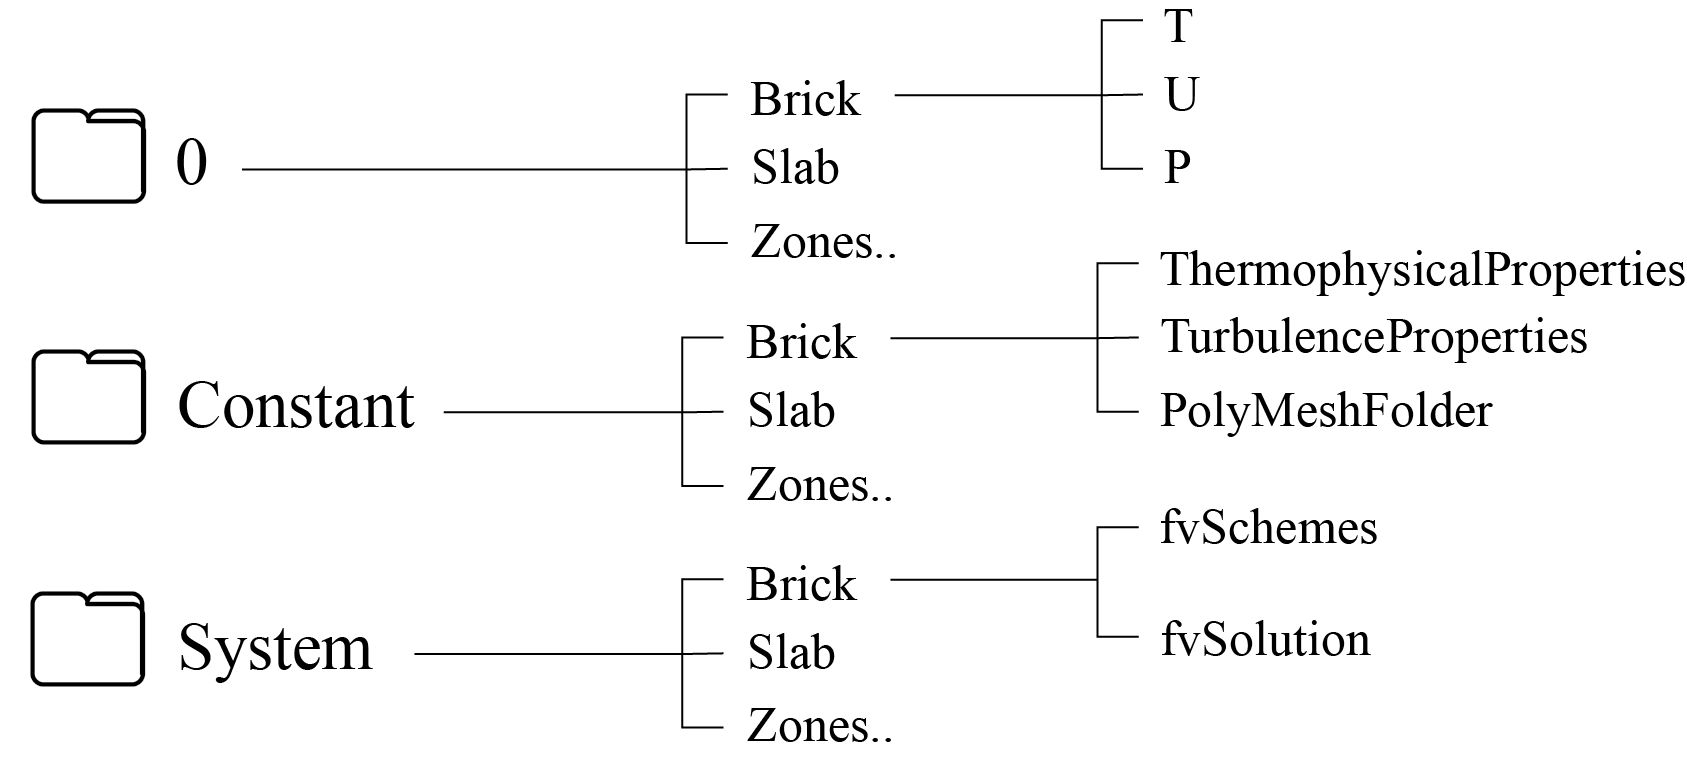
\includegraphics[width=0.77\columnwidth]{Figures/constc.png}
\hspace{0.7cm}
\caption[OF Case Contents]{OF case folders to run. Where (zones..) represent a folder for each zone in the case.}
\label{constc}
\end{figure}





\subsection{Running The Case}    
 
We discuss the selected solver capabilities to run the numerical simulation. The goal is to solve heat transfer in solid and liquid regions between air regions and the selected geometry. Using QuickField software to solve for 3D heat transfer showed some limitations where it does not consider the air regions. However, our approach using \gls{OF} includes the integration between air and solids to produce more accurate results. 

\begin{figure}[tbh] 
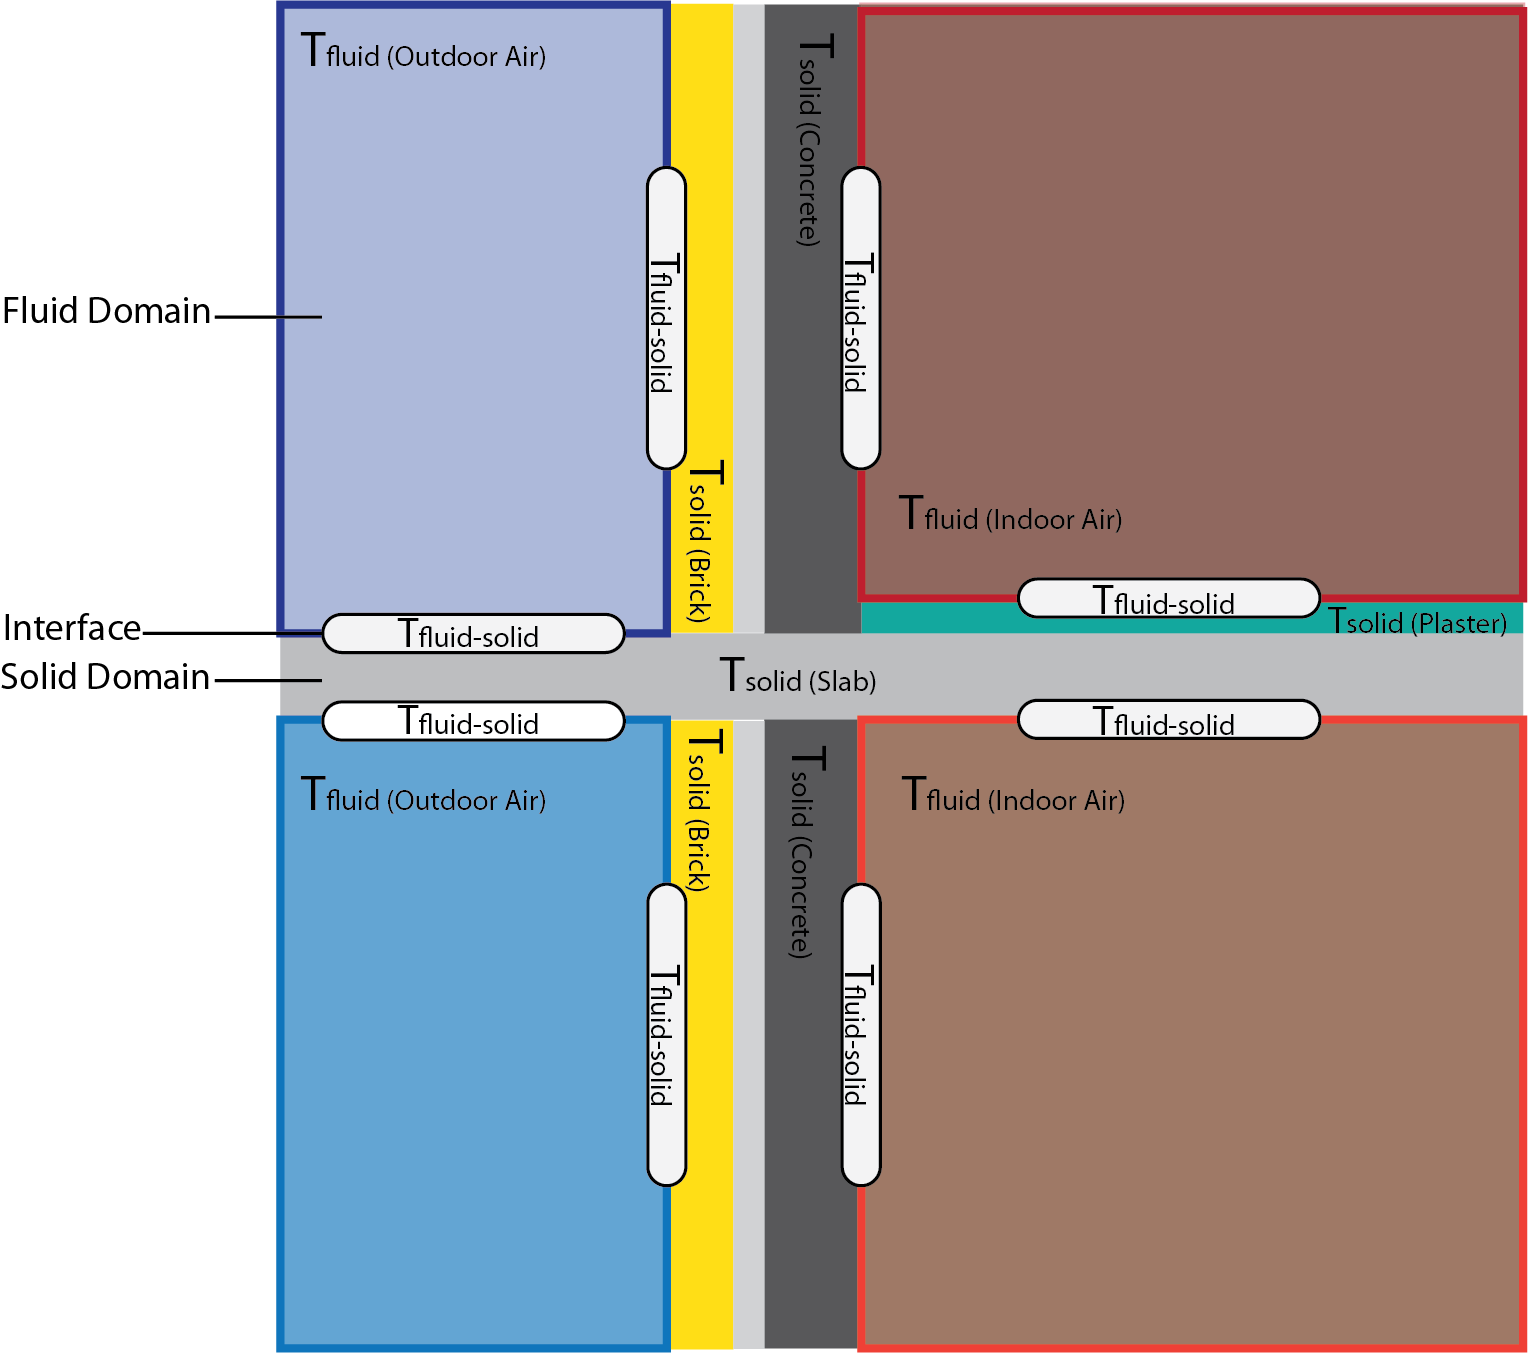
\includegraphics[width=0.77\columnwidth]{Figures/conductive.png}
\hspace{0.7cm}
\caption[3D Interfaces]{Vertical section of the validation case shows convection and conduction.}
\label{interface}
\end{figure}

\begin{figure}[tbh]
\centering

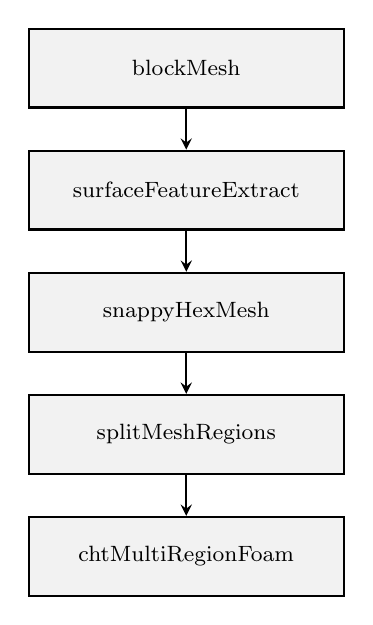
\begin{tikzpicture}[node distance=1.55cm, thick, every node/.style={scale=1}]
% Define nodes
\footnotesize
\node (blockMesh) [block] {blockMesh};
\node (surfaceFeatureExtract) [block, below of=blockMesh] {surfaceFeatureExtract};
\node (snappyHexMesh) [block, below of=surfaceFeatureExtract] {snappyHexMesh};
\node (splitMeshRegions) [block, below of=snappyHexMesh] {splitMeshRegions};
\node (chtMultiRegionFoam) [block, below of=splitMeshRegions] {chtMultiRegionFoam};
% Connect nodes with arrows
\draw [arrow] (blockMesh) -- (surfaceFeatureExtract);
\draw [arrow] (surfaceFeatureExtract) -- (snappyHexMesh);
\draw [arrow] (snappyHexMesh) -- (splitMeshRegions);
\draw [arrow] (splitMeshRegions) -- (chtMultiRegionFoam);
\end{tikzpicture}


\caption[OF Executables]{Order of executables for multiregion case setup with  \gls{OF} v2306.}
\label{fig:order-of-executables}
\end{figure}






\ref{fig:order-of-executables} illustrates the executables that need to be executed in order for a multiregion case.
The \textit{blockMesh} utility generates parametric meshes incorporating grading and curved edges. 
The meshes are created based on the specifications outlined in a dictionary file named \textit{blockMeshDict}  within the case directory.
\textit{surfaceFeatureExtract} extracts the surface features and then records them in a file.      
\textit{snappyHexMesh} is a utility in \gls{OF} that generates 3D meshes with hexahedra from STL surfaces, iteratively refining while maintaining surface conformity, shown in \ref{meshsteps}.
\textit{splitMeshRegions} divides the mesh into separate regions. Each region consists of cells reachable without crossing boundary faces, including cell zones.
\textit{chtMultiRegionFoam} is a solver for both steady and transient fluid flow, with solid heat conduction and conjugate heat transfer. The equations for each system variable are solved, and the solutions from the preceding equations are inserted into the subsequent ones. For instance, fluid-solid coupling solves fluid equations first, using the previous iteration's solid temperature to set fluid temperature boundary conditions. Then we solved the fluid equations using the same method. The simulation using this process continued until convergence at time step 400.
    
\begin{figure}[htb]
     \centering
    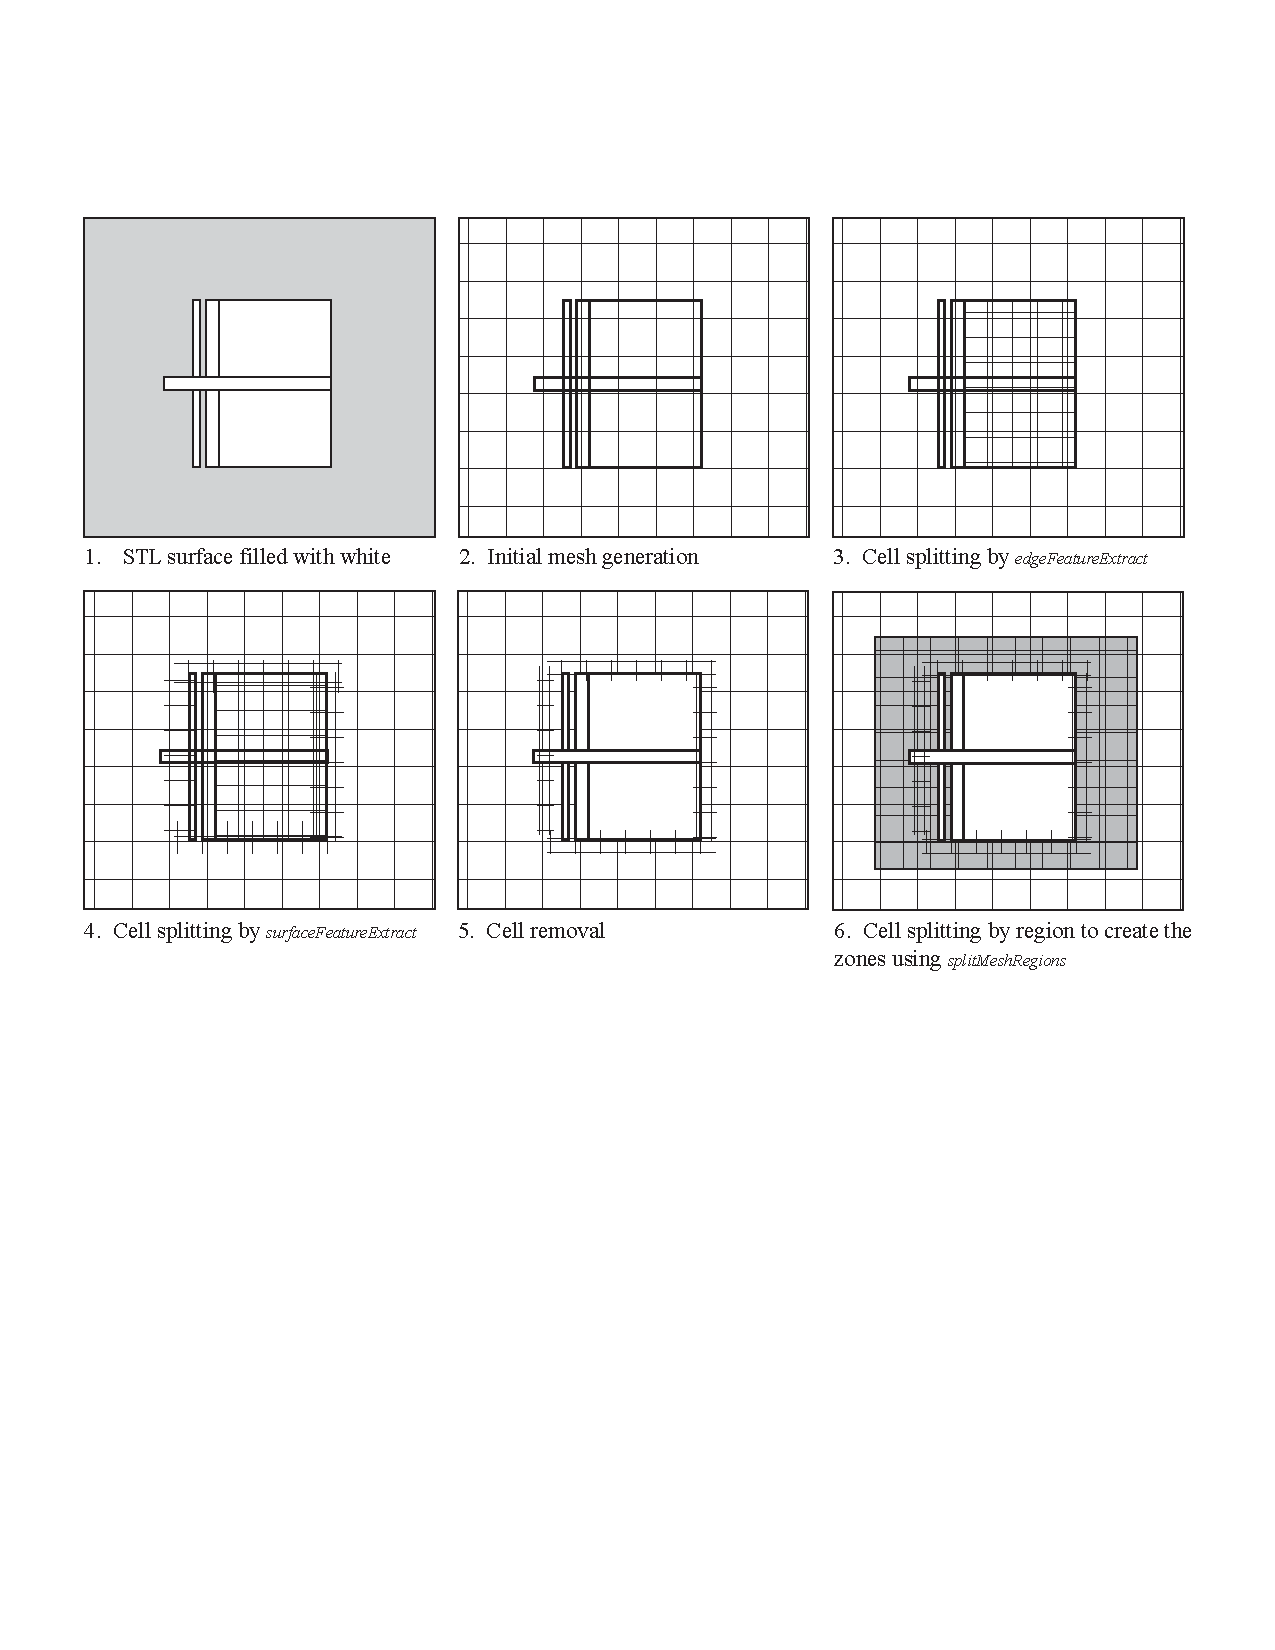
\includegraphics[trim=1cm 11cm 1cm 3cm, clip, width=1\linewidth]{Figures/snappyhex.pdf}
     \caption[Mesh Creation Steps]{Visualization of the steps and executables to create the mesh step-by-step.}
   \label{meshsteps}
 \end{figure}


%\clearpage
\subsection{Post-processing}
After running the simulation until convergence, multiple text files of $T$, $P$, and $U$ are solved for each region. There are two methods to post-process and visualize the resulting data. The first method is using Paraview to visualize the outcome and process the results. The second method is \gls{OF}'s post-process command, first, select the probing locations using \gls{GH} automation components to automatically write the post-processing file and measure the data, then plot the data to compare the validation case temperatures with our results. 



\afterpage{\clearpage}
\section{Results}

This section discusses the results of key experimental results of our ongoing research. 
\Cref{paraview} \textbf{(a)} visualizes the simulation temperature output, including the air (fluid) regions. Whereas
\Cref{paraview} \textbf{(b)} shows the geometry excluding air, which represents the temperature distributions. The resulting temperatures are shown in the plot in \cref{fig:validation-plots}. The plot includes the QuickField outputs and our \gls{OF} simulation along the z-axis from $z= 1.2$ to $z=2.2$ (the red line shown in \cref{paraview} \textbf{(a)}) and represents non-linear progression as a result of the different specific heat capacities and thermal conductivity of the materials. The peak in z=1.8 refers to the temperature of the slab, which can be modified by readjusting the slab model and re-simulating it. 



\begin{figure}[htb]
    \centering
    \textbf{(a)}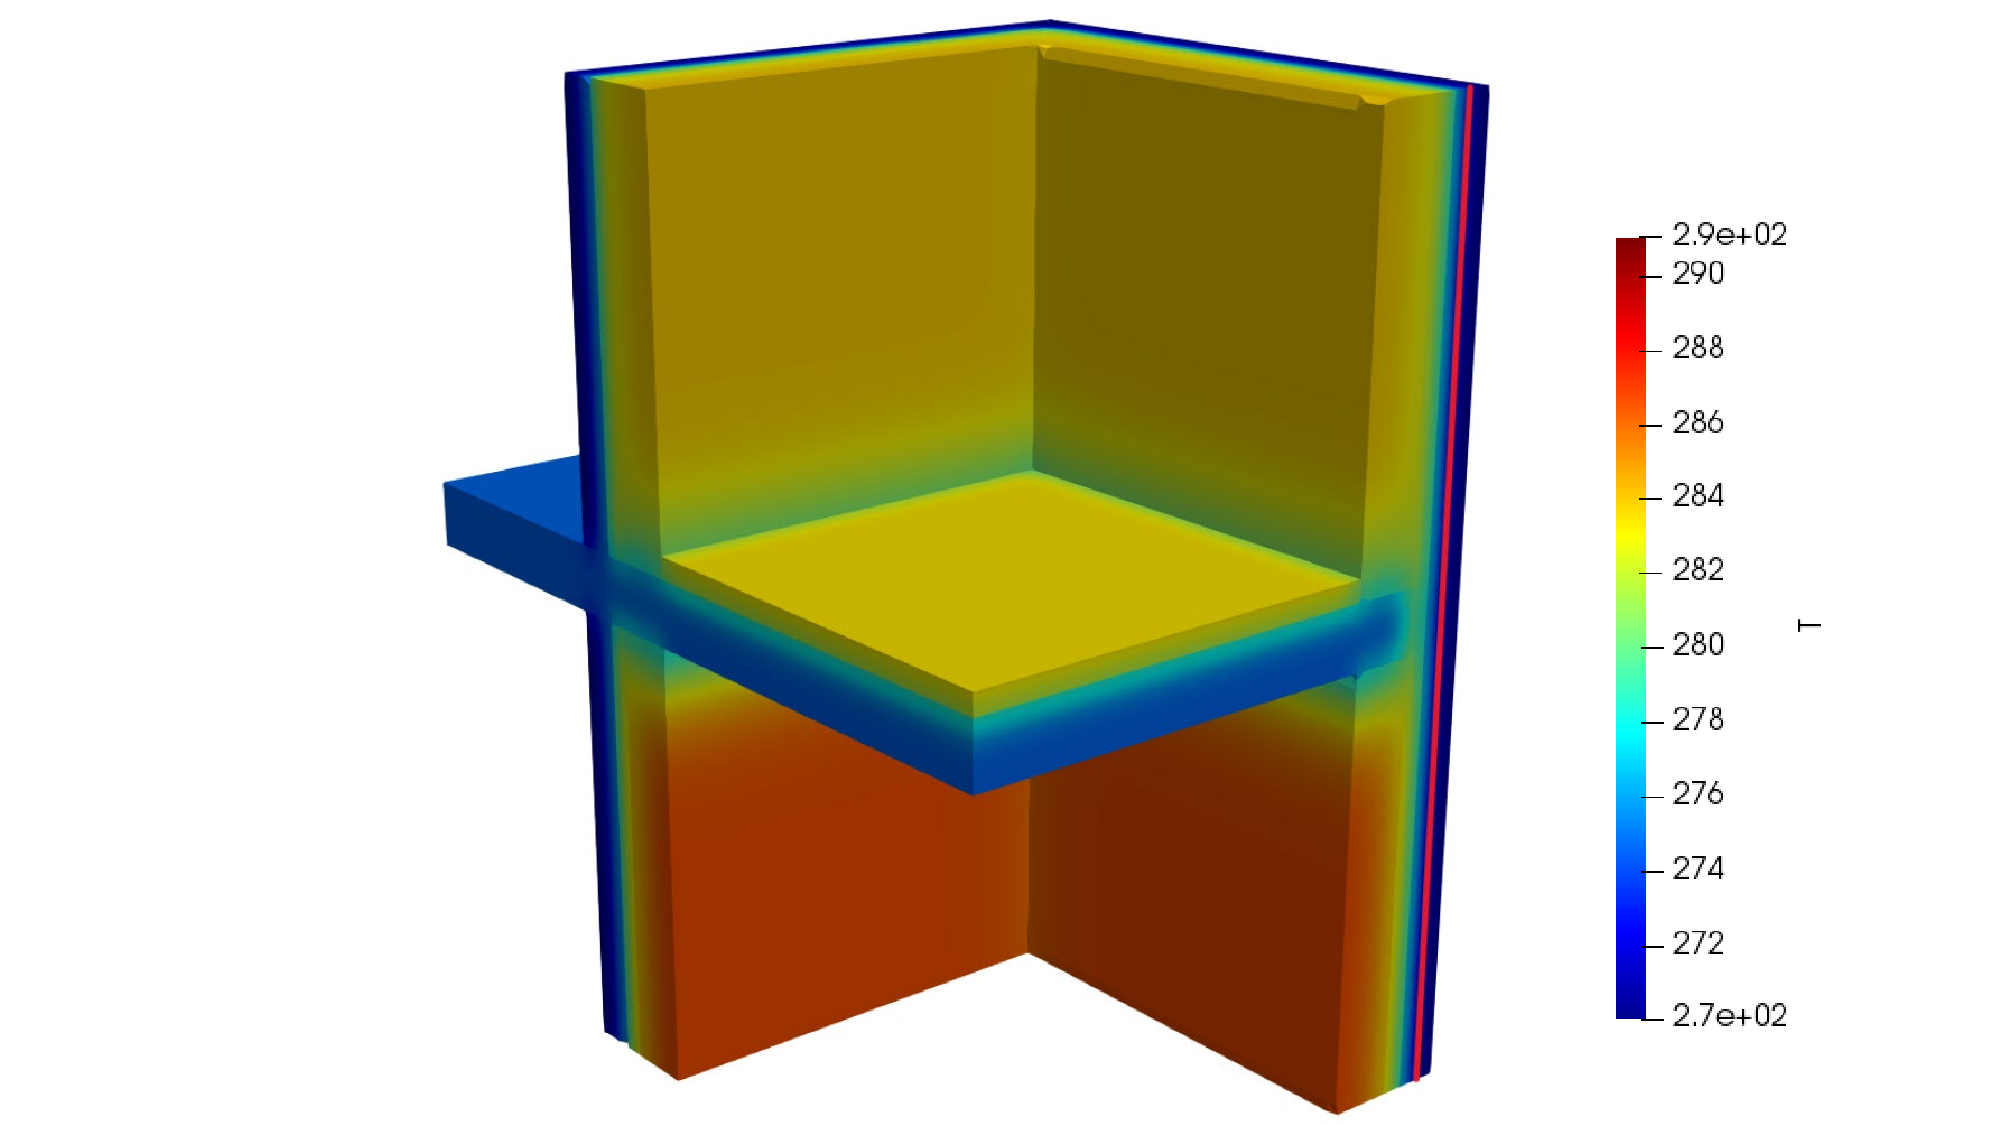
\includegraphics[trim=5cm 0cm 4.5cm 0cm, clip, width=0.70\linewidth]{Figures/newvalleg.pdf}
    \textbf{(b)}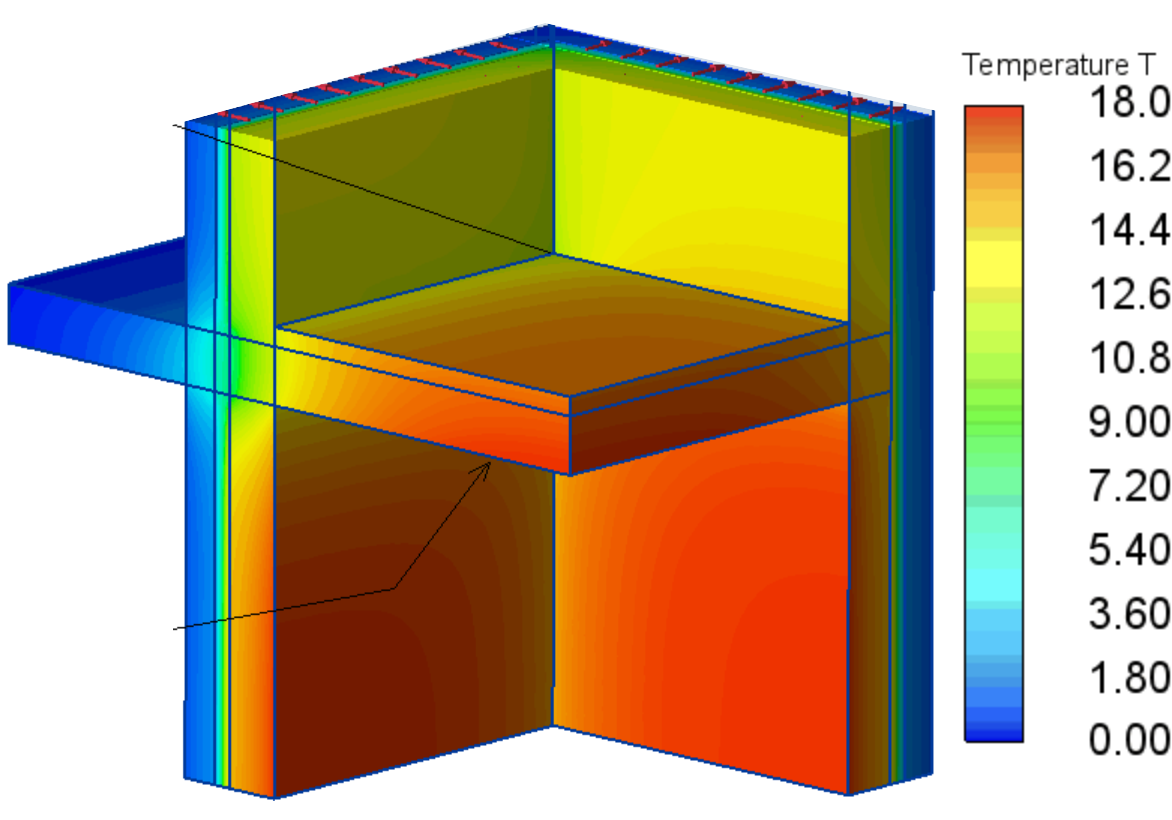
\includegraphics[width=0.65\columnwidth]{Figures/ValidationCaseClean.png}
\hspace{0.7cm}
    \caption[3D Validation Visualization]{\textbf{(a)} \gls{OF} case 3D results. \textbf{(b)} Quickfield validation results.}
    \label{paraview}
\end{figure}



\begin{figure}[htb] 
\centering
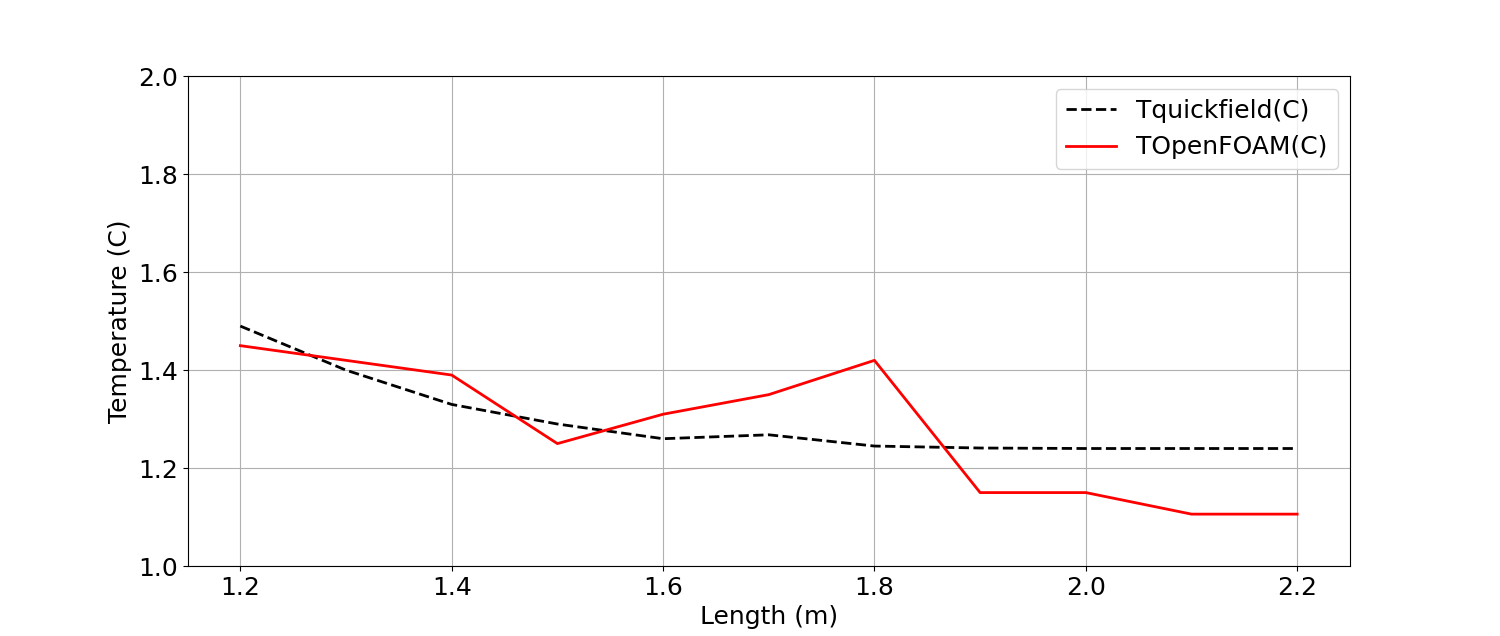
\includegraphics[width=1\columnwidth]{Figures/valpl2.png}
\hspace{0.7cm}
\caption{3D Validation Plots.}
\label{fig:validation-plots}
\end{figure}





\afterpage{\clearpage}
\section{Discussion}


The workflow presented in this thesis can be considered an extension of the work by \citeauthor{kastner2020solving} \cite{kastner2020solving}. 
The findings highlight several issues in the field, such as cost-prohibitive software, and disconnection between architectural modeling with heat transfer modeling software. 
The results illustrate the capabilities of using Rhinoceros and Grasshopper to simplify the pre-processing and post-processing steps to run the 3D heat transfer simulation in \gls{OF}. 
The simulation focuses on convective and conductive heat transfer for a 3D heat transfer problem. The 3D validation case study consists of two-floor corner sections separated by a concrete slab with a balcony. This case study was selected because it has the potential to present many challenges and problems in heat transfer, such as thermal bridges.


\subsection{Challenges}
\subsubsection{SIGFPE Error}
In some cases when changing or rescaling the geometry in Rhino, running the solver results in a signal floating-point error (SIGFPE), which might involve issues such as division by zero, floating-point underflow or overflow, integer overflow, etc. \cite{sigfpe}. However, in our case, the error occurs from divisions by zero and can be resolved in three ways depending on the circumstance. First, if the geometry in Rhino is re-scaled, the error can be resolved by recomputing the Grasshopper script. The second solution is to verify the boundary conditions in the $P$, and $P_{rgh}$ files, where they need to be absolute pressure and not relative when changing the \gls{OF} text files. The final solution is to recheck the boundary conditions and ensure that the zero gradient is properly assigned to the correct regions.


\subsubsection{Post-Processing}
Another challenge was to post-process the validation case via QuickField 6.6 (student version), which has several limitations compared to the \gls{OF} simulation discussed in this thesis. 
These include the inability to choose specific points to analyze temperature, limited visualization options, and no ability to adjust the density of points in the temperature plots. This made it difficult to compare specific temperature patterns.
QuickField 6.6 (student) does not allow selecting custom probing locations, limiting us to predefined ones.


\subsubsection{Slab Inaccuracy}
In the 3D validation case, the slab results demonstrate inaccuracies compared to the experimental case study. Despite the validation of the presented workflow of both the experimental design and the 3D case, the slab's behavior does not align as expected. An attempted solution involved changing the boundary condition at the $max_X$ boundary from $zeroGradient$ to $fixedValue$.
Although this adjustment slightly reduced the impact of the thermal bridge, it also introduced a larger issue by incorrectly representing heat transfer in the wall layer, as shown in Figure \ref{maxx}.

%gls/x, y, z

\begin{figure}[tb]
\centering
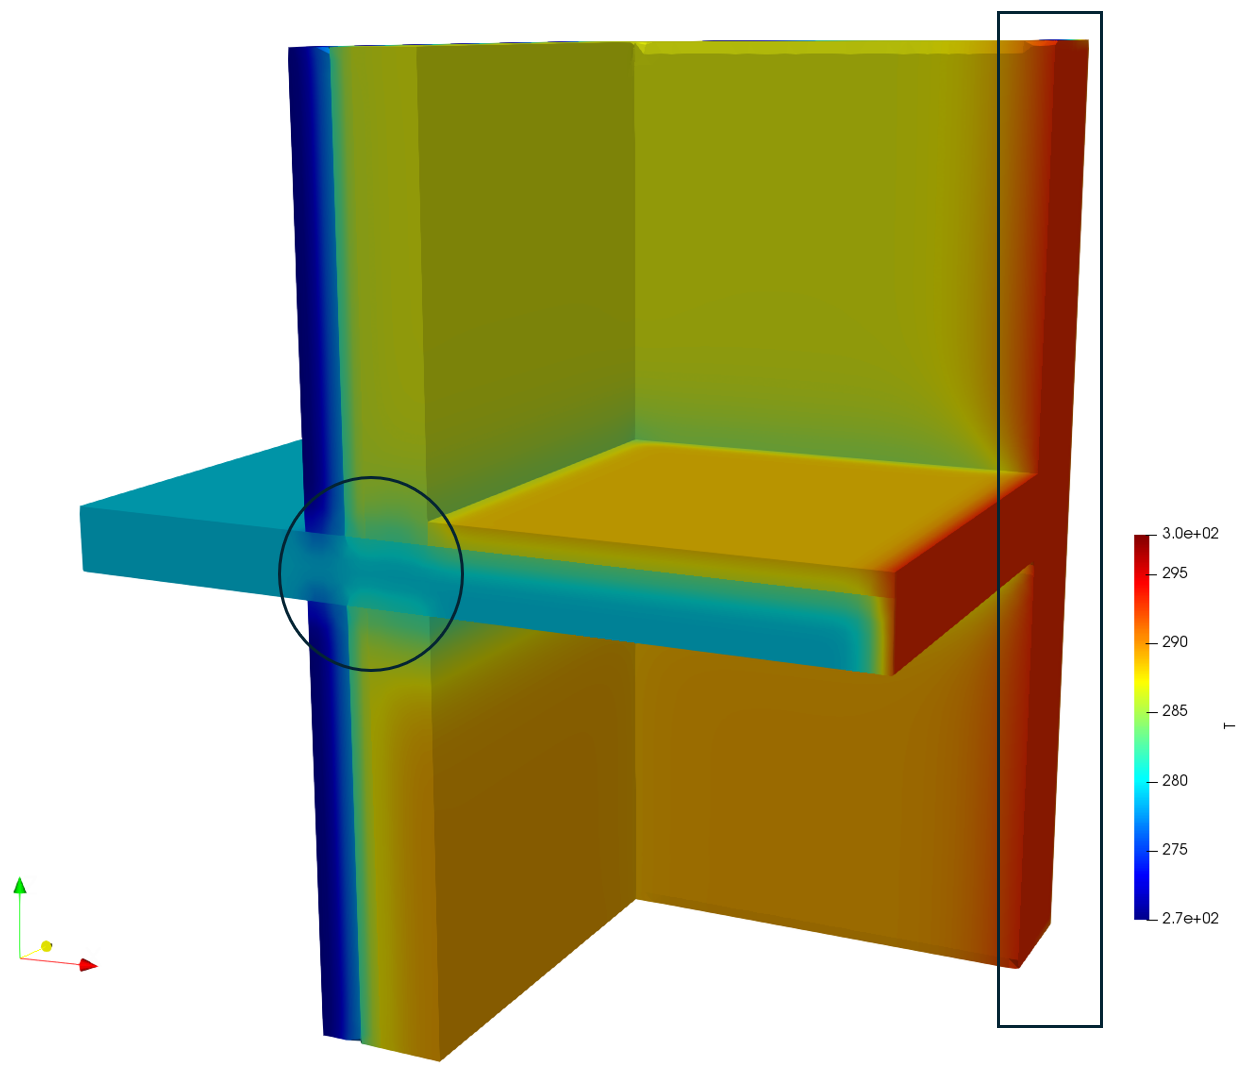
\includegraphics[width=0.75\columnwidth]{Figures/maxx.png}
\hspace{0.7cm}
\caption[Slab Validation]{Results of changing boundary conditions, highlighting a wall layer error and reduced thermal bridge.}
\label{maxx}
\end{figure}

Since these results do not fully consider the effect of thermal break between the exterior and interior sections of the slab, the following solutions may address the problem. The first suggested solution is to adjust the slab to have non-uniform initial conditions. This can be achieved by creating a $setFieldsDict$ file in the system folder. Using $setFieldsDict$, one can specify different initial temperatures for the exterior and interior sections of the slab, leading to a more accurate representation of the heat transfer. Another possible solution is to remodel the geometry and divide the slab into two distinct regions. This approach allows better control over the thermal distribution and potentially improves the accuracy of the simulation results.

Both of these solutions aim to correct the inconsistencies caused by incorrect boundary conditions and thermal bridging effects, leading to more accurate results in the 3D validation case.

\subsection{Experimental Design}
In the experimental design section of this thesis, U-value and heat flux sensors were used to log the temperatures and heat flux for a brick wall for 74 hours. The results were documented in 10-second increments throughout the three days. To validate the results of the experiment with the simulation \gls{OF}, three time steps were chosen from the experimental results to be simulated in three separate steady state heat transfer cases shown in \ref{table2d}, \ref{error2d}, and \ref{fig:expr}. However, the experiment can be easily validated by setting up one transient heat transfer case using the same \textit{chtMultiRegionFoam} solver. To leverage the solver's transient state capabilities, a time-dependent boundary condition must be provided. 


\subsection{Expanding Capabilities} %\todo{call this differently, this sounds weird}
Additional capabilities to the simulation is enabling the users to visualize the thermal comfort in the space (temperature of fluid in the space). In addition, the use of the adaptable \textit{chtMultiRegionFoam} solver is designed to simulate complex heat transfer scenarios for various applications. It is suitable for analyzing and helping model the performance of heating and cooling systems in the HVAC industry. In addition, the workflow can be used to assess solar heat gain, analyze heat exchangers, predict condensation, and assess insulation performance. Moreover, integration into Rhino significantly reduces the time required to simulate 3D heat transfer by condensing the steps to achieve the simulation.




    %\clearpage
\chapter{Conclusion}
This thesis presents an automated integration between GH, Rhino, and OF workflow to simulate 3D heat transfer in architectural applications. 
By utilizing OF, this research fills a critical gap in current design practices and is capable of improving energy-efficient building design and data-driven material selection. 

This 3D heat transfer workflow can help in building performance decisions such as suitable material selection, thermal comfort analysis, and insulation.
The stated aspects all are determined using data-driven decisions by either using machine learning, optimization, or analysis software. Thus, having an integrated 3d heat transfer tool incorporated from the preliminary design phase to the schematic phase is essential to ultimately reduce the building's operational and embodied carbon emissions. 

Future work in this field includes packaging the GH automation to provide a user-friendly GH plug-in. Also, using the same CHT solver to simulate for transient state 3D heat transfer or predict condensation and moisture. By leveraging advanced computational tools like OpenFOAM and integrating them seamlessly into existing design software offers a practical solution to a challenge and provides architects with the means to make informed decisions easier and faster. 

\section{Research Outcomes}
First, this research won the Kendeda Microgrant featured in \cite{kendeda} where the funds were used to purchase the U-value measurement kit. https://research.gatech.edu/micro-research-grants-awarded
The outcomes of this simulation experiment were presented at the Kendeda Microgrant Symposium in Spring 2024. 
A condensed version of this thesis has been accepted for submission in the 2024 International Building Physics conference proceedings in Toronto, Canada \cite{ibpc}. 


%\vspace{0.15in}
%\small
%\nomenclature{\(CHT\)}{Conjugate Heat Transfer}
%\nomenclature{\(PCM\)}{Phase Changing Materials}
%\nomenclature{\(CAD\)}{Computer-aided design}
%\nomenclature{\(ASHRAE\)}{American Society of Heating, Refrigerating and Air-Conditioning Engineers}
%\nomenclature{\(C_p\)}{Specific heat capacity, \si{\joule\per\kilogram\per\kelvin}}
%\nomenclature{\(d\)}{Length, \si{\metre}}
%\nomenclature{\(h\)}{Heat transfer coefficient, \si{\watt\per\metre\squared\per\kelvin}}
%\nomenclature{\(k\)}{Thermal conductivity, \si{\watt\per\metre\per\kelvin}}
%\nomenclature{\(\Psi\)}{Linear thermal transm. coeff., \si{\watt\per\metre\per\kelvin}}
%\nomenclature{\(q\)}{Heat flux density, \si{\watt\per\metre\squared}}
%\nomenclature{\(U\)}{Thermal transmittance, \si{\watt\per\metre\squared\per\kelvin}}
%\nomenclature{\(T\)}{Temperature, \si{\celsius\kelvin}}
%\nomenclature{\(x,\ y,\ z\)}{Cartesian coordinates, \si{\metre}}

    
% The environment used here (theappendices) is a wrapper for the basic appendices environment which changes the appearance of the title page and the structure and appearance of the appendices in the table of contents and PDF bookmarks. The original functionality can be restored by simply removing the 'the' from the \begin{} and \end{} statements below.

\begin{theappendices}


\chapter{Experimental Equipment}



\begin{table}[tbh]
\begin{framed}  
\small
\setlist[itemize]{leftmargin=3.5mm}
\begin{itemize}[topsep=1pt,itemsep=1pt,partopsep=1pt, parsep=1pt]
    \item \textbf{Product:} gSKIN® KIT-2615C (calibrated)
    \item \textbf{Article Number:} A-163479
    \item \textbf{GSKIN® KIT Includes (For More Details Consult The Datasheets Of The Individual Products):}
    \begin{itemize}[topsep=0pt,itemsep=0pt,partopsep=0pt, parsep=0pt]
        \item Sensor: gSKIN®-XO 67 7C (30mm x 30mm)
        \item Logger: gSKIN® DLOG-4231
        \item Double-sided mounting tape (MOUNT-1235)
    \end{itemize}
    \item \textbf{Heat Flux:}
    \begin{itemize}[topsep=0pt,itemsep=0pt,partopsep=0pt, parsep=0pt]
        \item Range Min / Max [W/M²]: ±300
        \item Resolution [W/M²]: $<$ 0.22
    \end{itemize}
    \item \textbf{Temperature Accuracy [°C]:}
    \begin{itemize}[topsep=0pt,itemsep=0pt,partopsep=0pt, parsep=0pt]
        \item ±0.5 (-10…+46 °C)
        \item ±2.0 (-55…+125 °C)
    \end{itemize}
    
    \item \textbf{Min. Sensor Sensitivity} 
    7.0 (sensor calibration data already loaded onto logger for simple and fast plug-and-play measurements)
    \item \textbf{Data Storage Capacity \# Measurements]:} $<$ 2’000’000
    \item \textbf{Battery Lifetime [Days]:} $<$ 30 at lowest measurement frequency (2/d). Rechargeable.
    \item \textbf{Software:} Installation - SW sent by email / via download link
    \item \textbf{Logger Dimensions (mm):} 52 x 20 x 15
    \item \textbf{Bit Resolution [Bits]:} 12
    \item \textbf{Operation Modes:} Autonomous / Live
    \item \textbf{Operating Temperature Range Min/Max [°C]:} -40 / 100 (-25 / 65 for Logger)
    \item \textbf{Operating System:} Windows 2000 / XP / Vista / 7 / 8
    \item \textbf{Calibration Accuracy $\mp$\%} 3 (Sensor calibration data already loaded onto logger for simple and fast plug-and-play measurements)
    \item \textbf{Calibration Temperature Range Min/Max [°C]:} -30 / 70
    \item \textbf{Heat Flux Sensor Cable Length [m]:} 1.5 (with connector)
    \item \textbf{Temperature Sensor 1 / 2 Cable Length [m]:} 5.0 / 1.0
    \item \textbf{Measurement Frequency:} 1/s to 1/h
    \item \textbf{Computer Interface:} USB     
\end{itemize}
\end{framed}
\caption{U-value measurement kit specifications by GreenTeg.}
\label{tab:u-value-measurement-kit}
\end{table}


\footnotesize
\singlespacing
\chapter{T File 0 Example}
\begin{lstlisting}[language=c++, caption=OF dictiorary in $0/Brick/T$]
/*-------------------*- C++ -*----------------------------------*\
| =========    |                                                 |
| \\      /  F | OpenFOAM: The Open Source CFD Toolbox           |
|  \\    /   O | Version:  2306                                  |
|   \\  /    A | Website:  www.openfoam.com                      |
|    \\/     M |                                                 |
\*--------------------------------------------------------------*/
FoamFile
{
    version     2.0;
    format      ascii;
    arch        "LSB;label=32;scalar=64";
    class       volScalarField;
    location    "0/";
    object      T;
}
// * * * * * * * * * * * * * * * * * * * * * * * * * * * * * * * //

dimensions      [0 0 0 1 0 0 0];

internalField   uniform 270;

boundaryField
{
Brick_to_Brick
{
            type compressible::turbulentTemperatureRadCoupledMixed;
            value  uniform 273;
            Tnbr T;
            K solidThermo;
            kappaMethod solidThermo;
            
}
...
\end{lstlisting}




\singlespacing
\chapter{File Constant Example}
\begin{lstlisting}[language=c++, caption=OF dictiorary in $constant/Brick/thermoPhysicalProperties$]
/*-------------------*- C++ -*----------------------------------*\
| =========    |                                                 |
| \\      /  F | OpenFOAM: The Open Source CFD Toolbox           |
|  \\    /   O | Version:  2306                                  |
|   \\  /    A | Website:  www.openfoam.com                      |
|    \\/     M |                                                 |
\*--------------------------------------------------------------*/
FoamFile
{
    version     2.0;
    format      ascii;
    class       dictionary;
    object      thermophysicalProperties;
}
// * * * * * * * * * * * * * * * * * * * * * * * * * * * * * * * //
thermoType
{
    type            heSolidThermo;
    mixture         pureMixture;
    transport       constIso;
    thermo          hConst;
    equationOfState rhoConst;
    specie          specie;
    energy          sensibleEnthalpy;
  }
mixture
{
    specie
    {
        molWeight   12;
    }
    transport
    {
        kappa   80;
    }
    thermodynamics
    {
        Hf      1;
        Cp      1060;
    }
    equationOfState
    {
        rho     1600;
    }
}
// *********************************************************** //
\end{lstlisting}






\singlespacing
\chapter{File System Example}
\begin{lstlisting}[language=c++, caption=OF dictiorary in $system/Brick/fvSolution$]
/*-------------------*- C++ -*----------------------------------*\
| =========    |                                                 |
| \\      /  F | OpenFOAM: The Open Source CFD Toolbox           |
|  \\    /   O | Version:  2306                                  |
|   \\  /    A | Website:  www.openfoam.com                      |
|    \\/     M |                                                 |
\*--------------------------------------------------------------*/
FoamFile
{
    version     2.0;
    format      ascii;
    class       dictionary;
    object      fvSolution;
}
// * * * * * * * * * * * * * * * * * * * * * * * * * * * * * * * //

solvers
{
    "(rho|rhoFinal)"
    {
        solver          PCG;
        preconditioner  DIC;
        tolerance       1e-7;
        relTol          0;
    }

    p_rgh
    {
        solver           GAMG;
        tolerance        1e-7;
        relTol           0.01;
        smoother         GaussSeidel;
    }

    p_rghFinal
    {
        $p_rgh;
        tolerance        1e-7;
        relTol           0;
    }

\end{lstlisting}




\singlespacing
\chapter{Write T File Example}

We used a mesh user dictionary approach to build the geometry pipeline within Grasshopper.

\begin{lstlisting}[language=c++, caption= Code to handle OF dictionary in $0/Brick/T$]
...
m.UserDictionary["name"]);
m.UserDictionary["type"]);
m.UserDictionary["temp"]);
...
\end{lstlisting}







\normalsize
\singlespacing
\chapter{Specific Heat Capacity Solution (Brick Example)}
\begin{equation}
\begin{aligned}
\Delta T &= 15^\circ \text{C} \\
d &= 100 \, \text{mm} = 0.1 \, \text{m} \\
A &= 1300 \times (950 + 50 + 50 + 950) \, \text{mm}^2 \\
A &= 1300 \times (2000) \, \text{mm}^2 = 2.6 \, \text{m}^2 \\
Q &= \frac{k \cdot A \cdot \Delta T}{d} \\
&\text{solve for the specific heat capacity ($C_p$):} \\
C_p &= \frac{Q \cdot d}{k \cdot A \cdot \Delta T} \\
Q &= k \cdot A \cdot \frac{\Delta T}{d} \\
Q &= 0.7 \, \text{W/m.K} \times 2.6 \, \text{m}^2 \times 15^\circ \text{C} / 0.1 \, \text{m} \\
Q &= 27 \, \text{W} \\
C_p &= \frac{27 \, \text{W} \times 0.1 \, \text{m}}{0.7 \, \text{W/m.K} \times 2.6 \, \text{m}^2 \times 15^\circ \text{C}} \\
C_p &= \frac{2.7 \, \text{J}}{2.55 \, \text{J/K}} \\
C_p &\approx 1.06 \, \text{kJ/kg.K} \\
&\text{So, the specific heat capacity of the brick is approximately} \, 1.06 \, \text{kJ/kg.K} \\
&\text{To convert to J/kg.K:} \\
C_p &= 1.06 \, \text{kJ/kg.K} \times 1000 \\
C_p &= 1060 \, \text{J/kg.K}
\end{aligned}
\label{appendcp}
\end{equation}




































\end{theappendices}
    \makeBibliography
    % Vita should only be included for PhD candidates.

\begin{vita}

Maryam Almaian...

\end{vita}
\end{thesisbody}

\end{document}
